\chapter{Proof of Concept}
\label{sec:proof_of_concept}

% -------------------------------------------------------------------------------

% parameers: xlabel, center
\newcommand{\fuzzyTreeNode}[2]{
    \begin{tikzpicture}
        \begin{axis}%
            [
                title = {Fuzzy Split: $#1 \leq #2$},
                width=4.5cm,
                height=3cm,
                axis lines=center,
                xlabel={#1},
                x label style={at={(axis description cs:0.9,-0.1)},anchor=north},
                ylabel=$\mu$,
                y label style={at={(axis description cs:0.5,1)},anchor=south},
                xmin=-5,
                xmax=5,
                xtick={},
                xticklabels= {},
                ytick={},
                yticklabels={},
                extra x ticks={0},
                extra x tick labels={#2},
                ymax=1,
                samples=50,
                extra y ticks={1},
                every axis plot/.append style={thick}
            ]
            \addplot[red]  {sigmoid(x,0,-1)};
            \addplot[blue] {sigmoid(x,0,1)};
            \node[anchor=center, red] at (axis cs:-2.9,0.6) {$\mu_{\text{#1smaller#2}}$};
            \node[anchor=center, blue] at (axis cs:3.1,0.6) {$\mu_{\text{#1greater#2}}$};
        \end{axis}

    \end{tikzpicture}
}

\newcommand{\fuzzyTreeLeaf}[1]{
    \begin{tikzpicture}
        \begin{axis}%
            [
                title = {Class: #1},
                width=3.25cm,
                height=2.25cm,
                axis lines=center,
                xlabel={$\text{class}$},
                x label style={at={(axis description cs:0.6,-0.3)},anchor=west},
                ylabel=$\mu$,
                y label style={at={(axis description cs:0.5,1)},anchor=south},
                xmin=-5,
                xmax=5,
                xtick={},
                xticklabels= {},
                ytick={},
                yticklabels={},
                extra x ticks={0},
                extra x tick labels={#1},
                ymax=1,
                samples=10,
                extra y ticks={1},
                every axis plot/.append style={thick}
            ]
            \addplot[black]  {gaussian(x,0,1)};
        \end{axis}

    \end{tikzpicture}
}

% parameers: xlabel, center
\newcommand{\crispTreeNode}[2]{
    \begin{tikzpicture}
        \begin{axis}%
            [
                title = {Crisp Split: $#1 \leq #2$},
                width=4.5cm,
                height=3cm,
                axis lines=center,
                xlabel={#1},
                x label style={at={(axis description cs:0.9,-0.1)},anchor=north},
                ylabel=$\mu$,
                y label style={at={(axis description cs:0.5,1)},anchor=south},
                xmin=-5,
                xmax=5,
                xtick={},
                xticklabels= {},
                ytick={},
                yticklabels={},
                extra x ticks={0},
                extra x tick labels={#2},
                ymin=-0.1,
                ymax=1.1,
                samples=50,
                extra y ticks={1},
                every axis plot/.append style={thick}
            ]
            \addplot[red,domain=-5:-0.6] {step(x,0,-1)};
            \addplot[blue,domain=0.6:5] {step(x,0,1)};
            \addplot[red,domain=0.6:5] {step(x,0,-1)};
            \addplot[blue,domain=-5:-0.6] {step(x,0,1)};

            \node[draw,draw=black,circle,inner sep=1pt,minimum width=3pt,thick] at (axis cs:0,1) {};
            \node[draw,draw=black,circle,inner sep=1pt,minimum width=3pt,thick] at (axis cs:0,0) {};

            \node[anchor=center, red] at (axis cs:-2.9,0.6) {$#1 \leq #2$};
            \node[anchor=center, blue] at (axis cs:3.1,0.6) {$#1 > #2$};
        \end{axis}

    \end{tikzpicture}
}


% -------------------------------------------------------------------------------

In this chapter, we present a proof of concept for the fuzzy tuning technique. We will develop a set of linguistic variables and fuzzy rules to predict the optimal configuration parameters for \texttt{\gls{mdflexible}} simulations.

\section{Creating the Knowledge Base}

One of the hardest parts of developing a fuzzy system is creating the knowledge base, as it typically requires a very deep understanding of the system to be able to create meaningful rules. However, there also exist methods to use a data-driven approach to create the knowledge base automatically. This is especially useful as those methods don't require any prior expert knowledge about the system. But regardless of the way the knowledge base is created, it is still possible to manually evaluate and adjust the rules to add manual expert knowledge to the system. Using such data-driven methods can be a good starting point for creating a fuzzy system, as it can provide a good initial set of rules that can be further refined by experts.

There are several methods to automatically create and tune fuzzy systems based on data. Some of the most common methods include genetic algorithms \todo{Add references to the methods}, particle swarm optimization, and decision trees.
In this work, we will use a decision tree aproach proposed by Crockett et al.~\cite{CROCKETT20062809} to create the knowledge base for the fuzzy system. This proposed method uses machine learning to first train a classical decision tree on the dataset and then converts the decision tree into a fuzzy decision tree which can then be used to extract the linguistic variables and fuzzy rules.


\section{Decision Trees}

Decision trees are very popular machine learning algorithms that are used for classification and regression tasks. They work by recursively partitioning the input using axis-parallel splits~\cite{10.5555/2380985}, in such a way that the resulting subsets are as pure as possible. There are several algorithms to train decision trees, such as ID3, C4.5, CART, and many others, but they all work by the principle of minimizing the \textit{impurity} of the resulting subsets. Decision trees are supervised learning algorithms, which means that they require labeled data to train.

A key feature of decision trees is their interpretability. This makes them a good choice for creating the initial knowledge base for a fuzzy system, as it is very easy for a human expert to understand and refine the rules created by the decision tree with additional knowledge.

Since decision trees directly partition the input space into regions with different classes, they can also be easyily represented by their decision surface (given that the dimensionality of the input space is low enough). The decision surface of a decision tree is a piecewise constant function that assigns the predicted class to each region of the input space. An example decision tree and its decision surface are shown in \autoref{fig:decisionTreeExample} and \autoref{fig:decisionBoundaryExample}.

% Image of a decision tree
\begin{multicols}{2}
    \begin{figure}[H] % [H] for HERE
        \centering
        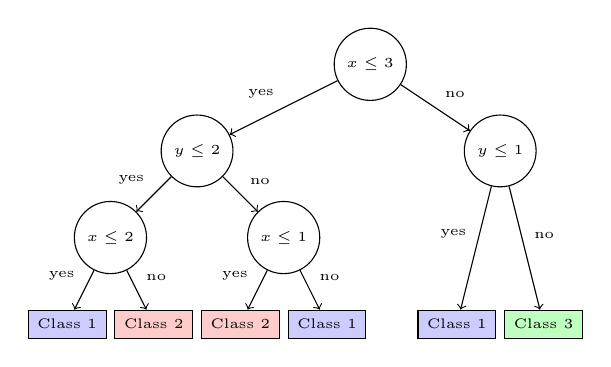
\begin{tikzpicture}[scale=1.1,font=\tiny]
            \node [circle,draw] (A) at (0,0) {$x \leq 3$};
            \node [circle,draw] (B) at (-2,-1) {$y \leq 2$};
            \node [circle,draw] (C) at (1.5,-1) {$y \leq 1$};
            \node [circle,draw] (D) at (-3,-2) {$x \leq 2$};
            \node [circle,draw] (E) at (-1,-2) {$x \leq 1$};

            \node [rectangle,draw,fill=blue!20] (F) at (-3.5,-3) {Class 1};
            \node [rectangle,draw,fill=red!20] (G) at (-2.5,-3) {Class 2};
            \node [rectangle,draw,fill=red!20] (H) at (-1.5,-3) {Class 2};
            \node [rectangle,draw,fill=blue!20] (I) at (-0.5,-3) {Class 1};
            \node [rectangle,draw,fill=blue!20] (J) at (1,-3) {Class 1};
            \node [rectangle,draw,fill=green!25] (K) at (2,-3) {Class 3};

            \draw[->] (A) -- (B) node [midway, left, above left] {yes};
            \draw[->] (A) -- (C) node [midway, right, above right] {no};
            \draw[->] (B) -- (D) node [midway, left, above left] {yes};
            \draw[->] (B) -- (E) node [midway, right, above right] {no};

            \draw[->] (C) -- (J) node [midway, left, above left] {yes};
            \draw[->] (C) -- (K) node [midway, right, above right] {no};

            \draw[->] (D) -- (F) node [midway, left, above left] {yes};
            \draw[->] (D) -- (G) node [midway, right, above right] {no};

            \draw[->] (E) -- (H) node [midway, left, above left] {yes};
            \draw[->] (E) -- (I) node [midway, right, above right] {no};

        \end{tikzpicture}

        \caption[Decision tree used for the example]{An example decision tree for a dataset with two features $x$ and $y$. There are three distinct classes in the dataset}
        \label{fig:decisionTreeExample}
    \end{figure}

    \columnbreak    % start next column

    \begin{figure}[H]
        \centering
        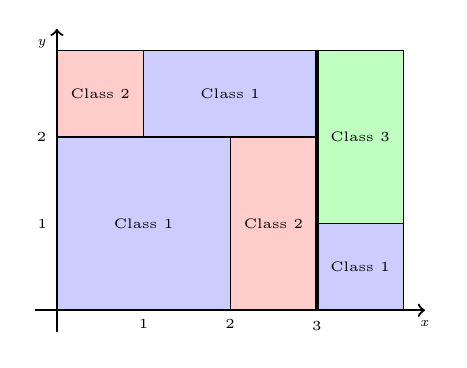
\begin{tikzpicture}[scale=1.1,font=\tiny]

            \draw[fill=red!20] (0,2) -- (1,2) -- (1,3) -- (0,3) -- cycle;

            \draw[fill=blue!20] (1,2) -- (3,2) -- (3,3) -- (1,3) -- cycle;

            \draw[fill=blue!20] (0,0) -- (2,0) -- (2,2) -- (0,2) -- cycle;
            \draw[fill=red!20] (2,0) -- (3,0) -- (3,2) -- (2,2) -- cycle;

            \draw[fill=blue!20] (3,0) -- (4,0) -- (4,1) -- (3,1) -- cycle;
            \draw[fill=green!25] (3,1) -- (4,1) -- (4,3) -- (3,3) -- cycle;

            \draw[->, thick] (-0.25,0) -- (4.25,0) node [below] {\textit{x}};
            \draw[->, thick] (0,-0.25) -- (0,3.25) node [below left] {\textit{y}};

            % decision lines

            \draw[line width=1.5pt,] (3,0) node [below] {3}  -- (3,3) ;
            \draw[line width=1pt] (0,2) node [left] {2} -- (3,2);

            \draw[] (2,0) node [below] {2}-- (2,2);

            \node [below] at (1,0) {1};

            \node [left] at (0,1) {1};

            % area labels
            \node [] at (0.5,2.5) {Class 2};
            \node [] at (2,2.5) {Class 1};

            \node [] at (1,1) {Class 1};
            \node [] at (2.5,1) {Class 2};


            \node [] at (3.5,2) {Class 3};
            \node [] at (3.5,0.5) {Class 1};

        \end{tikzpicture}
        \caption[Decision surface of the example decision tree]{The decision surface of the decision tree from \autoref{fig:decisionTreeExample} on $\mathcal{D}=[0,4]\times[0,3]$. }
        \label{fig:decisionBoundaryExample}
    \end{figure}
\end{multicols}



\section{Fuzzy Decision Trees}


Fuzzy decision trees are a generalization of classical decision trees that allow for fuzzy logic to be used in the decision-making process. This extension allows to eliminate the crisp decision boundaries of classical decision trees and instead use fuzzy sets at each node of the tree to calculate the contribution of each branch to the final decision. This allows for a more flexible decision-making process that can take into account the uncertainty of the input data and the splits. Contrary to classical decision trees, which follow a single path from the root to a leaf node, fuzzy decision trees explore all possible paths at the same time and make a final decision by aggregating the results of all paths using fuzzy logic. This is possible, as each node in a fuzzy decision tree can fuzzily assign how much each of its children should contribute to the final decision.

\section{Converting a Decision Tree into a Fuzzy Inference System}


In this section, we will demonstrate how to convert a classical decision tree into a fuzzy inference system using the fictional decision tree from \autoref{fig:decisionTreeExample} as an example.

The conversion of a classical decision tree to a fuzzy decision tree is done by replacing the crisp decision boundaries (e.g., $x \leq 3$) at each internal node with fuzzy membership functions. Those membership functions should have the same semantics as the crisp decision boundaries, but instead of returning a binary value of wheter to continue down the left or right branch, they return a value in the range $[0,1]$ that specifies to which degree each branch should be taken. The shape of the membership functions can be chosen arbitrarily, but since the decision should be one-sided, typical choices include complementary \texttt{sigmoid}-shaped functions.
An obvious choice for the membership functions is to use \texttt{sigmoid} functions with a center at the crisp decision boundary as this maintains the semantics of the branch. Crockett et al.~\cite{CROCKETT20062809} suggested defining symetric sigmoid functions on the interval $[t-n\cdot \sigma, t+n\cdot \sigma]$ where $t$ is the crisp decision boundary, $\sigma$ is the standard deviation of the attribute, and $n$ is a parameter that can be adjusted to control the \emph{width} of the membership function. The \emph{width} of the membership function describes the interval where there is a significant change in the membership value. Outside of this interval, the membership value is close to 0 or 1, depending on the side of the interval.

The value of $n$ is typical chosen from the interval $n\in [0,5]$ as otherwise the membership function can become too wide, weakening the decision-making process ~\cite{CROCKETT20062809}. In this work we will use $n=2$ as a default value.

By using a data dependent \emph{width} of the membership functions, it is possible to fully automate the conversion of a decision tree into a fuzzy decision tree which we will utilize in this work.


The conversion of a crisp decision boundary into a fuzzy decision boundary is shown in \autoref{fig:fuzzyMembershipFunctions} using the example split $x \leq 3$.



\begin{figure}[h]
    \centering
    \begin{tikzpicture}[scale=2,font=\tiny]
        \node [rectangle,rounded corners,draw,inner sep=2pt] (A) at (0.5,0) {
            \crispTreeNode{x}{3}
        };

        \node [rectangle,rounded corners,draw,inner sep=2pt] (B) at (3.5,0) {
            \fuzzyTreeNode{x}{3}
        };

        \path[draw=black, line width=1mm, -{Triangle[length=4mm, bend]}]
        (1.5,0) to [bend left] (2.5,0);

        \path[draw=white, line width=0.5mm, -{Triangle[length=3.25mm, bend, angle'=60]}, shorten >= 0.5mm, shorten <= 0.25mm]
        (1.5,0) to [bend left] (2.5,0);

    \end{tikzpicture}
    \caption[Conversion of crisp tree node into fuzzy tree node]{Conversion of a crisp decision surface to a fuzzy decision surface. The crisp decision surface $x \leq 3$ is replaced by two \texttt{sigmoid} membership functions \textcolor{red}{$\mu_{\text{xsmaller3}}$} and \textcolor{blue}{$\mu_{\text{xgreater3}}$} that specify to which degree the comparison is true or false. The \emph{width} of the membership function is data dependent and is determinend by $n\cdot \sigma = 2 \cdot \sigma$.}
    \label{fig:fuzzyMembershipFunctions}
\end{figure}


Once the internal nodes of the decision tree have been converted, the next step is to convert the leaf nodes of the decision tree to fuzzy leaf nodes, representing the class values. This is also done by replacing each crisp class value with a fuzzy membership function that assigns a degree of membership to the class. The shape of the membership functions can again be chosen arbitrarily, but we will use \texttt{gaussian} functions with a specific mean and variance. The placement of the different class-specific membership functions is very important, as it can heavily influence the defuzzification process for some defuzzification methods as fuzzy systems typically use a interpolation between the different class values to determine the final output. The resulting conversion of the decision tree to a fuzzy decision tree is shown in \autoref{fig:fuzzyDecisionTreeExample}.


\begin{figure}[h]
    \centering
    \begin{tikzpicture}[scale=2,font=\tiny]

        \node [rectangle,rounded corners,draw,inner sep=2pt] (A) at (0,0) {
            \fuzzyTreeNode{x}{3}
        };

        \node [rectangle,rounded corners,draw,inner sep=2pt] (B) at (-2,-1.5) {
            \fuzzyTreeNode{y}{2}
        };

        \node [rectangle,rounded corners,draw,inner sep=2pt] (C) at (1.5,-1.5) {
            \fuzzyTreeNode{y}{1}
        };

        \node [rectangle,rounded corners,draw,inner sep=2pt] (D) at (-3,-3) {
            \fuzzyTreeNode{x}{2}
        };

        \node [rectangle,rounded corners,draw,inner sep=2pt] (E) at (-1,-3) {
            \fuzzyTreeNode{x}{1}
        };


        \node [rectangle,rounded corners,draw,inner sep=2pt,fill=blue!20] (F) at (-3.5,-4.5) {
            \fuzzyTreeLeaf{1}
        };

        \node [rectangle,rounded corners,draw,inner sep=2pt,fill=orange!20] (G) at (-2.5,-4.5) {
            \fuzzyTreeLeaf{2}
        };

        \node [rectangle,rounded corners,draw,inner sep=2pt,fill=orange!20] (H) at (-1.5,-4.5) {
            \fuzzyTreeLeaf{2}
        };

        \node [rectangle,rounded corners,draw,inner sep=2pt,fill=blue!20] (I) at (-0.5,-4.5) {
            \fuzzyTreeLeaf{1}
        };

        \node [rectangle,rounded corners,draw,inner sep=2pt,fill=blue!20] (J) at (1,-4.5) {
            \fuzzyTreeLeaf{1}
        };

        \node [rectangle,rounded corners,draw,inner sep=2pt,fill=green!20] (K) at (2,-4.5) {
            \fuzzyTreeLeaf{3}
        };



        \draw[->] (A) -- (B) node [pos=.4, left, above left] {yes};
        \draw[->] (A) -- (C) node [pos=.4, right, above right] {no};

        \draw[->] (B) -- (D) node [pos=.8, left, above left] {yes};
        \draw[->] (B) -- (E) node [pos=.8, right, above right] {no};

        \draw[->] (C) -- (J) node [pos=.2, left, above left] {yes};
        \draw[->] (C) -- (K) node [pos=.2, right, above right] {no};

        \draw[->] (D) -- (F) node [pos=.6, left, above left] {yes};
        \draw[->] (D) -- (G) node [pos=.6, right, above right] {no};

        \draw[->] (E) -- (H) node [pos=.6, left, above left] {yes};
        \draw[->] (E) -- (I) node [pos=.6, right, above right] {no};
    \end{tikzpicture}

    \caption[Fuzzy decision tree created from the regular decision tree]{The fuzzy decision tree corresponding to the decision tree in \autoref{fig:decisionTreeExample}. Each internal node in the fuzzy decision tree uses two \texttt{sigmoid} membership functions (\textcolor{red}{$\mu_{\text{smaller}}$} and \textcolor{blue}{$\mu_{\text{greater}}$}) to specify to which degree the comparison is true or false. The leaf nodes use different \texttt{gaussian} membership functions centered around their class value.}

    \label{fig:fuzzyDecisionTreeExample}
\end{figure}

After the translation of the decision tree, all membership functions operating on the same variable can be combined into a single linguistic variable. Note that the specific shapes of the membership functions has been picked arbitrarily and can be adjusted to better fit the data. The resulting linguistic variables are shown in \autoref{fig:fuzzyDecisionTreeLinguisticVariables}.

\begin{figure}[H]
    \centering

    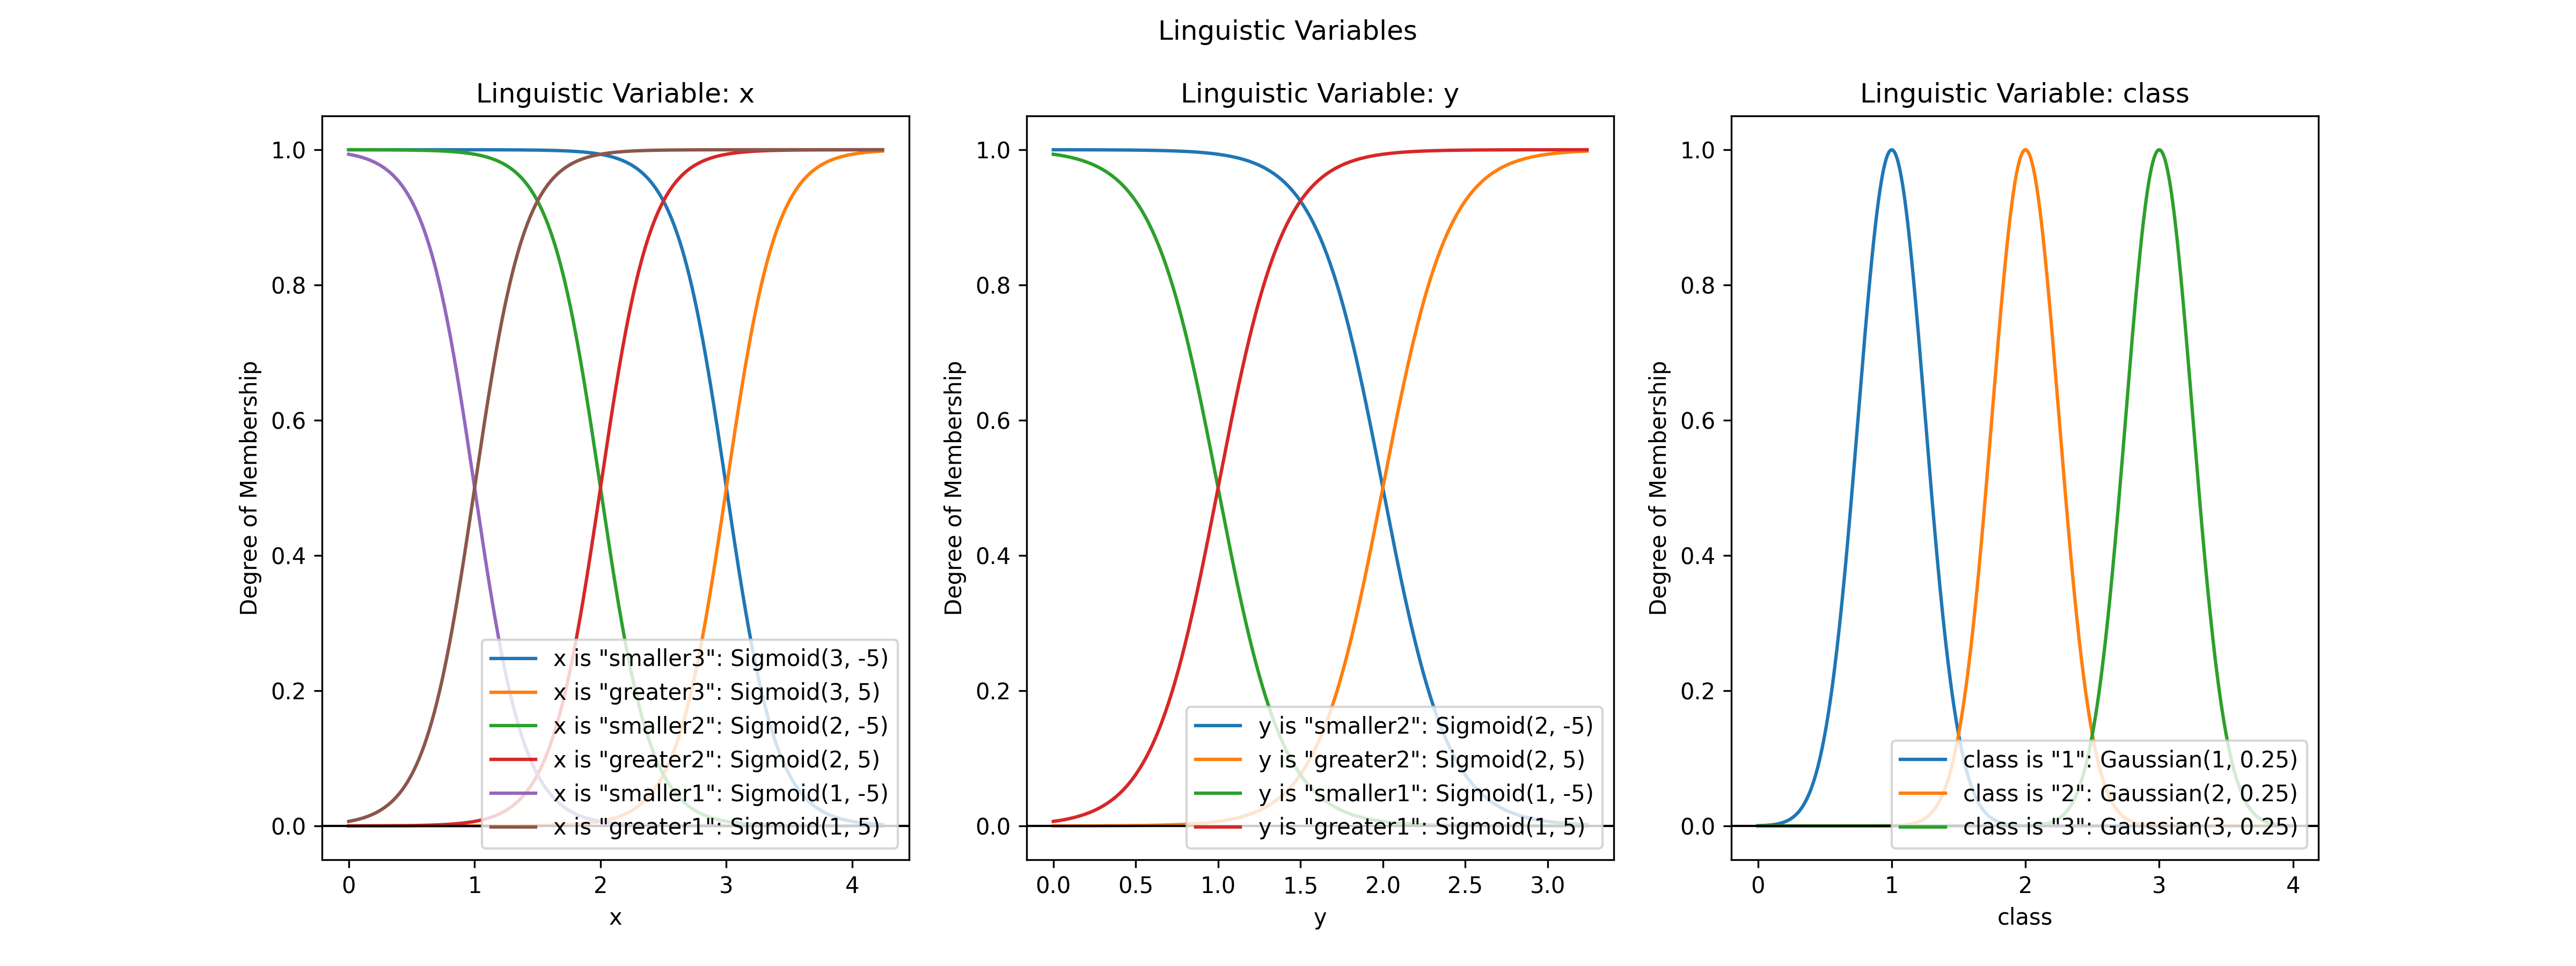
\includegraphics[width=\linewidth,trim={3.5cm 0 3.5cm 1cm},clip]{figures/ProofOfConcepts/fuzzy_sets.png}

    \caption[Linguistic variables for the converted fuzzy decision tree]{Linguistic variables used in the fuzzy decision tree in \autoref{fig:fuzzyDecisionTreeExample}. The standard deviation of the attributes is assumed to be $\sigma \approx 0.5$ such that the \emph{width} of the sigmoid membership functions is $n\cdot \sigma \approx 1$. The class values are assumed to be normally distributed and are places such that they dont overlap much.}
    \label{fig:fuzzyDecisionTreeLinguisticVariables}
\end{figure}

\subsubsection{Rule Extraction}

Once the fuzzy decision tree has been created, the next step is to extract the fuzzy rules from the tree. This can be done by traversing the tree in a depth-first manner and collecting the correct membership functions for each path along the way. Each connection between two internal nodes in the tree corresponds to a \texttt{AND} operation, while each final connection between an internal node and a leaf node corresponds to an \texttt{IMPLIES} operation. This implication then forms a rule for the fuzzy system.
This process esentially mimics the decision surface seen in \autoref{fig:decisionBoundaryExample}, as we create exactly one rule for each region of the decision surface. The rules extracted from the fuzzy decision tree in \autoref{fig:fuzzyDecisionTreeExample} are shown in \autoref{tab:fuzzyRulesExample}.

\newcommand{\is}{\textit{ is }}


\begin{table}[H]
    \centering
    \begin{tabular}{c|l|c}
        \textbf{Rule} & \textbf{Antecedent}                                                             & \textbf{Consequent} \\
        \hline
        1             & $x \is \text{smaller3} \land y \is \text{smaller2} \land x \is \text{smaller2}$ & $class \is 1$       \\
        2             & $x \is \text{smaller3} \land y \is \text{smaller2} \land x \is \text{greater2}$ & $class \is 2$       \\
        3             & $x \is \text{smaller3} \land y \is \text{greater2} \land x \is \text{smaller1}$ & $class \is 2$       \\
        4             & $x \is \text{smaller3} \land y \is \text{greater2} \land x \is \text{greater1}$ & $class \is 1$       \\
        5             & $x \is \text{greater3} \land y \is \text{smaller1}$                             & $class \is 1$       \\
        6             & $x \is \text{greater3} \land y \is \text{greater1}$                             & $class \is 3$       \\
    \end{tabular}
    \caption[Extracted fuzzy rules from the fuzzy decision tree]{Extracted fuzzy rules from the fuzzy decision tree in \autoref{fig:fuzzyDecisionTreeExample} in the format: $\textbf{IF} \text{ Antecedent } \textbf{THEN} \text{ Consequent }$}
    \label{tab:fuzzyRulesExample}
\end{table}

\subsubsection{Fuzzy Inference System}

With the linguistic variables and fuzzy rules extracted from the decision tree, we can now use them to create a fuzzy system that can predict the class of a new data point based on its features. Since the fuzzy system can be seen as a black box mapping continuous input features to continuous output classes
(see \autoref{fig:fuzzyInferenceSystem}), it is possible to visualize the decision surface of the fuzzy system by evaluating the membership functions of the rules for each point in the input space. This decision surface can then be used to understand the decision-making process of the fuzzy system and to identify possible errors in the rules or membership functions.


\begin{figure}[h]
    \centering
    \begin{tikzpicture}[scale=2,font=\small]

        \node [rectangle,rounded corners,draw,inner sep=2pt] (B) at (0,1.2) {
            Rules, Linguistic Variables \& Defuzzification Method
        };

        \node [rectangle,rounded corners,draw,inner sep=2pt] (A) at (0,0) {
            \begin{tikzpicture}[scale=2,font=\tiny]
                \begin{axis}%
                    [
                        title={\gls{fis}},
                        width=3.2cm,
                        height=2cm,
                        axis lines=center,
                        xmin=0,
                        xmax=4,
                        xlabel={$class$},
                        x label style={at={(axis description cs:1,0.2)},anchor=west},
                        ylabel=$\mu$,
                        y label style={at={(axis description cs:0,0.8)},anchor=east},
                        xtick={},
                        xticklabels= {},
                        ytick={},
                        yticklabels={},
                        ymax=1,
                        every axis plot/.append style={thick},
                        domain=0:4
                    ]
                    \addplot[blue, samples=17] {gaussian(x,1,0.2)};
                    \addplot[red,samples=15] {gaussian(x,2,0.2)};
                    \addplot[green,samples=17] {gaussian(x,3,0.2)};
                \end{axis}
            \end{tikzpicture}
        };

        \draw[->,thick] (B) -- (A);

        \draw[->,ultra thick] (-2.5,+0.2) -- (A) node [left, pos=0] {$x \in \mathbb{R}$};
        \draw[->,ultra thick] (-2.5,-0.2) -- (A) node [left, pos=0] {$y \in \mathbb{R}$};
        \draw[->,ultra thick] (A) -- (2.5,0) node [right, pos=1] {$class \in \mathbb{R}$};
    \end{tikzpicture}

    \caption[Fuzzy inference system created from the fuzzy decision tree seen as a black box]{The fuzzy inference system created from the fuzzy decision tree in \autoref{fig:fuzzyDecisionTreeExample} can be seen as a black box that maps continuous input features to continuous output classes.}

    \label{fig:fuzzyInferenceSystem}
\end{figure}

\subsubsection{Choice of Defuzzification Method}

The exact shape of the decision surface depends on the used defuzzification method. The most common choice is the \gls{cog} method, which calculates the $x$-position of the center of gravity of the resulting membership function.
However, using the \gls{cog} method can lead to undesired results when using nominal \todo{check} values for the output classes, as there is no concept of ordering among the values.
Without such an ordering, the interpolation between the different classes performed by methuds such as \gls{cog} is not meaningful and leads to bad predictions. In such cases, other methods such as the \gls{mom} method can be used instead. This method calculates the mean value of the maximum membership functions. In most cases this method will return exactly the center of the  membership function with the highest value and is therefore a good choice for nominal values. A direct comparison of the two methods on a critical datapoint is shown in \autoref{fig:fuzzySetForDataCOG} and \autoref{fig:fuzzySetForDataMOM}

\begin{multicols}{2}

    \begin{figure}[H]
        \centering
        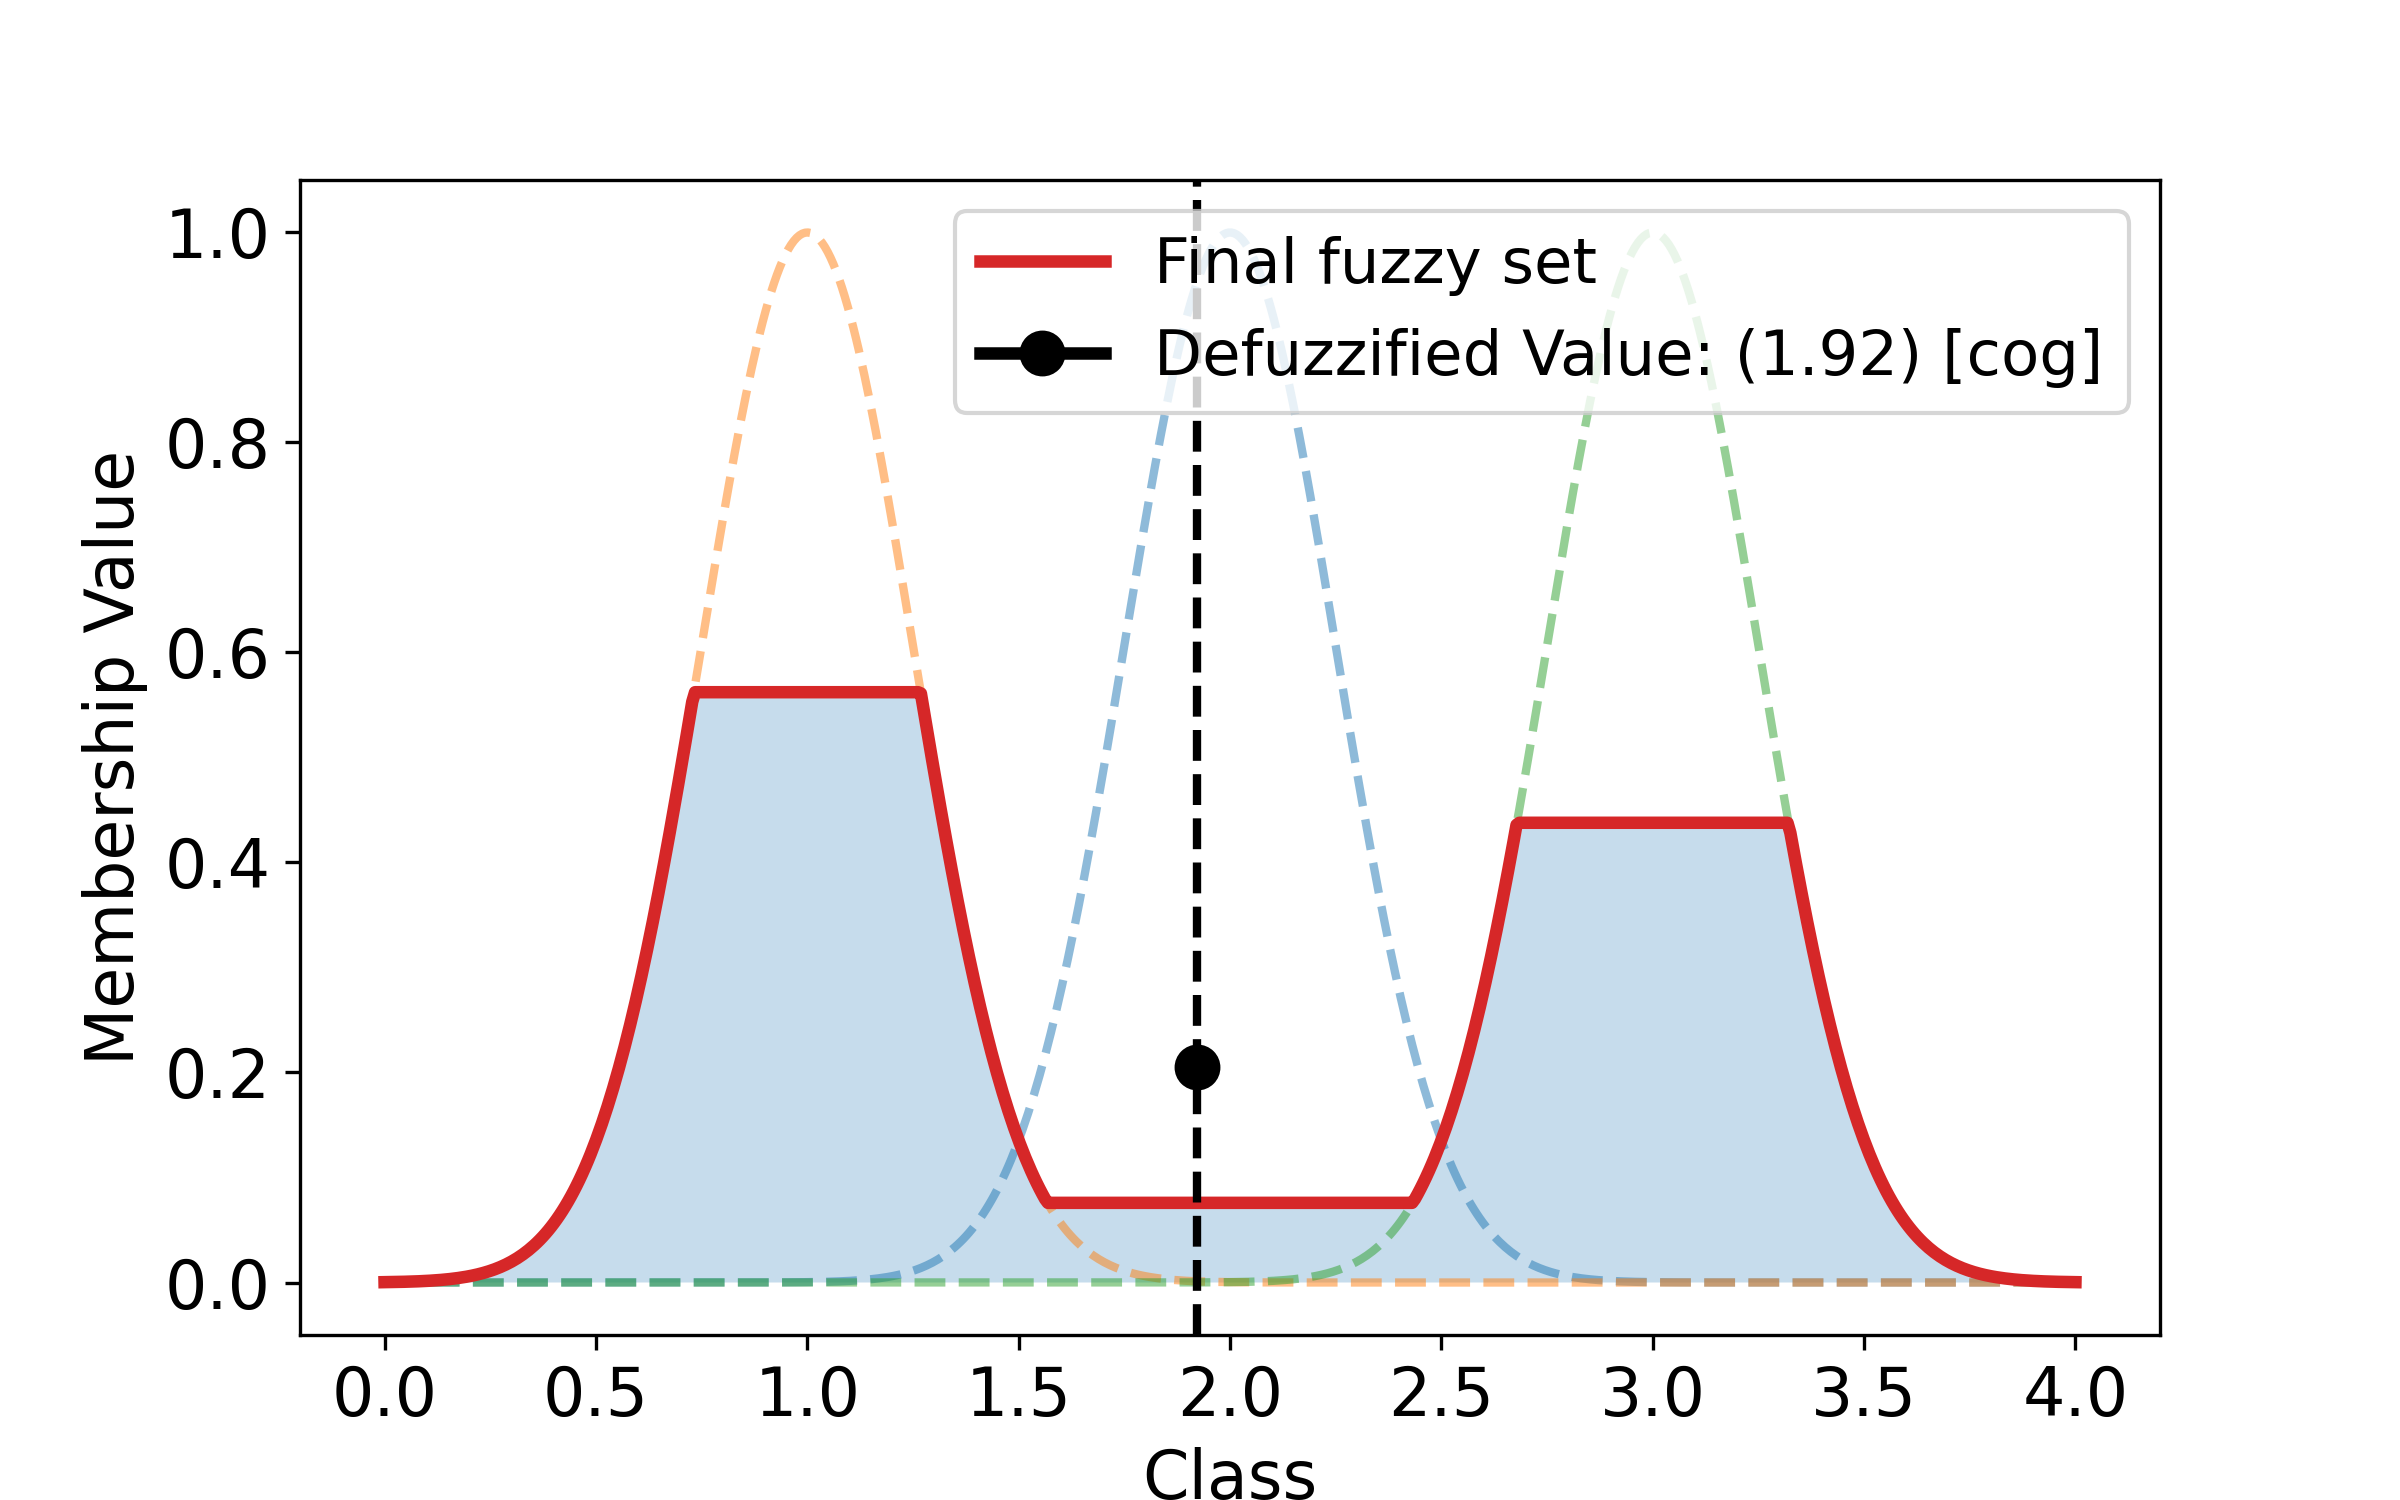
\includegraphics[width=0.9\columnwidth,trim={0 0 0 1cm},clip]{figures/ProofOfConcepts/fuzzy_set_for_data_cog.png}
        \caption[Resulting Fuzzy Set after applying the Rules on specific Data, COG Method]{Resulting fuzzy set after applying the rules from \autoref{tab:fuzzyRulesExample} on the data point $(x=2.95, y=2.5)$. There are clear peaks at the class values 1 and 3. The \gls{cog} method however returns Class 2, as it lies right in between the two peaks, turing the two good predictions into a bad one.}
        \label{fig:fuzzySetForDataCOG}
    \end{figure}

    \columnbreak

    \begin{figure}[H]
        \centering
        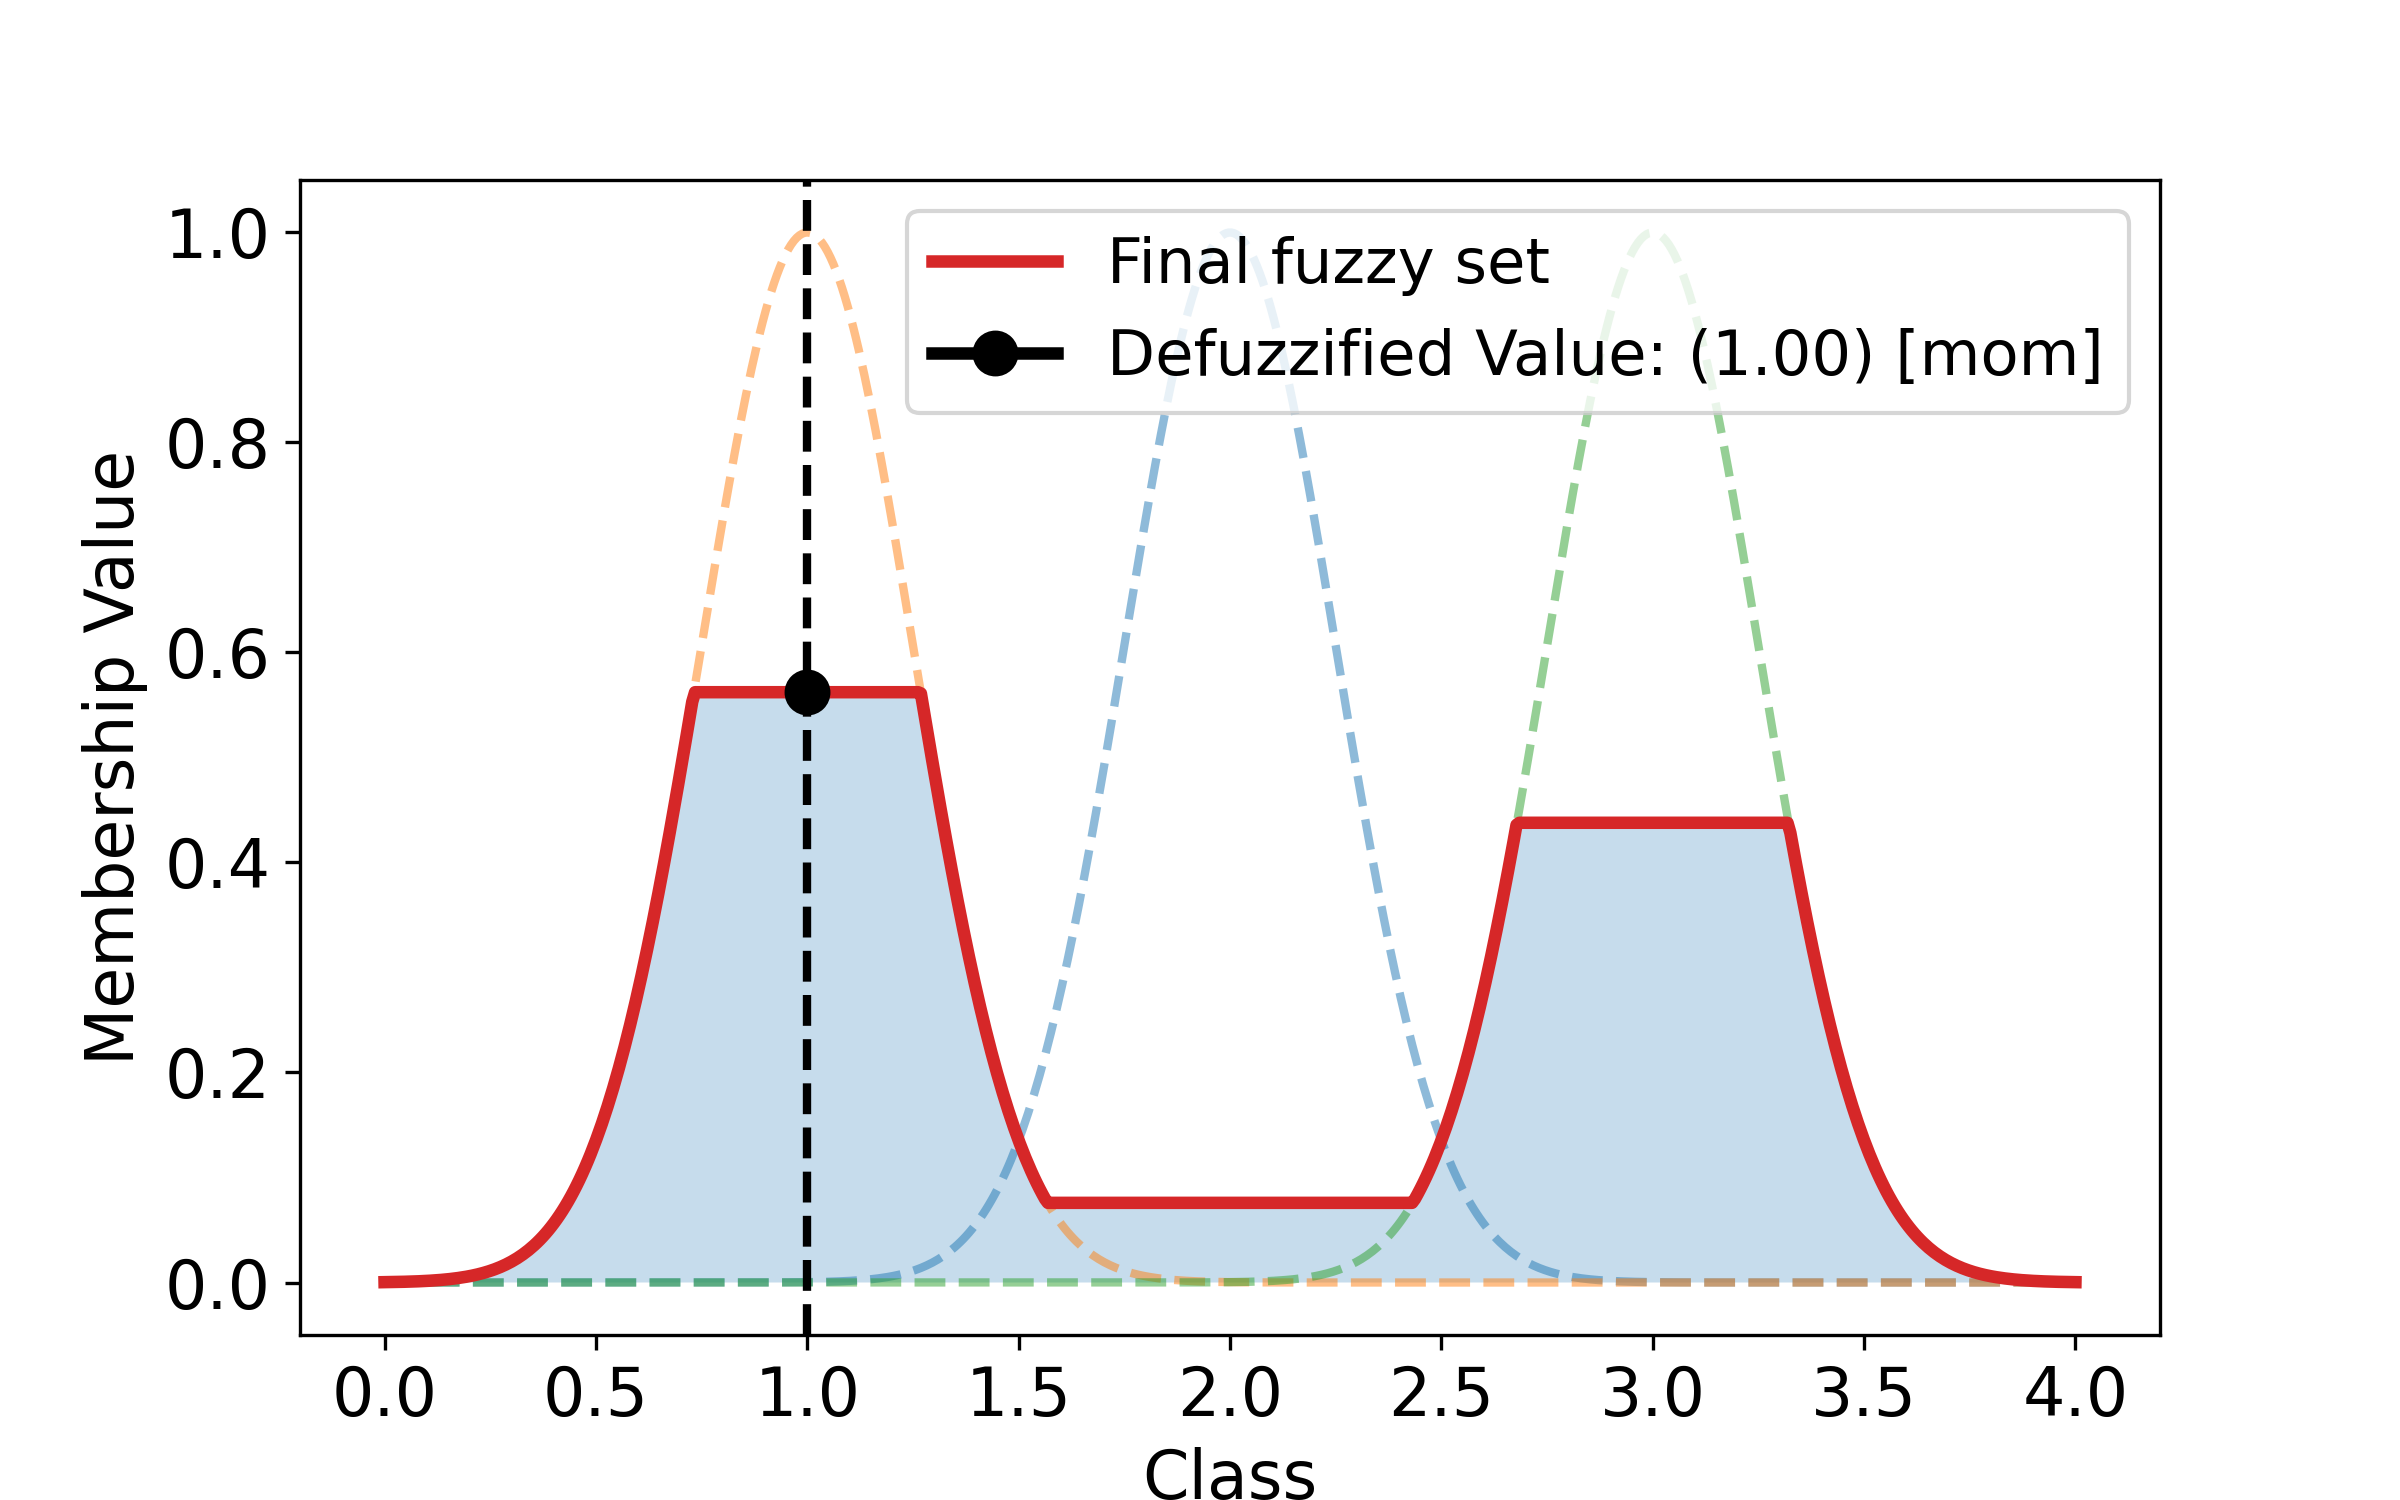
\includegraphics[width=0.9\columnwidth,trim={0 0 0 1cm},clip]{figures/ProofOfConcepts/fuzzy_set_for_data_mom.png}
        \caption[Resulting Fuzzy Set after applying the Rules on specific Data, MOM Method]{The \gls{mom} method returns the class value 1, as it is the mean of the two peaks at class values 1 and 3. This is a much better prediction than the one made by the \gls{cog} method.}

        \label{fig:fuzzySetForDataMOM}
    \end{figure}

\end{multicols}

It is also possible to calculate the whole decision surface of the fuzzy system by evaluating the membership functions of the rules for each point in the input space. Both the decision surface using the \gls{cog} and \gls{mom} defuzzification methods are shown in \autoref{fig:fuzzyDecisionSurfaceExampleCOG} and \autoref{fig:fuzzyDecisionSurfaceExampleMOM} respectively.

\begin{multicols}{2}
    \begin{figure}[H]
        \centering
        \begin{tikzpicture}
            \node[anchor=south west,inner sep=0] (image) at (0,0) { 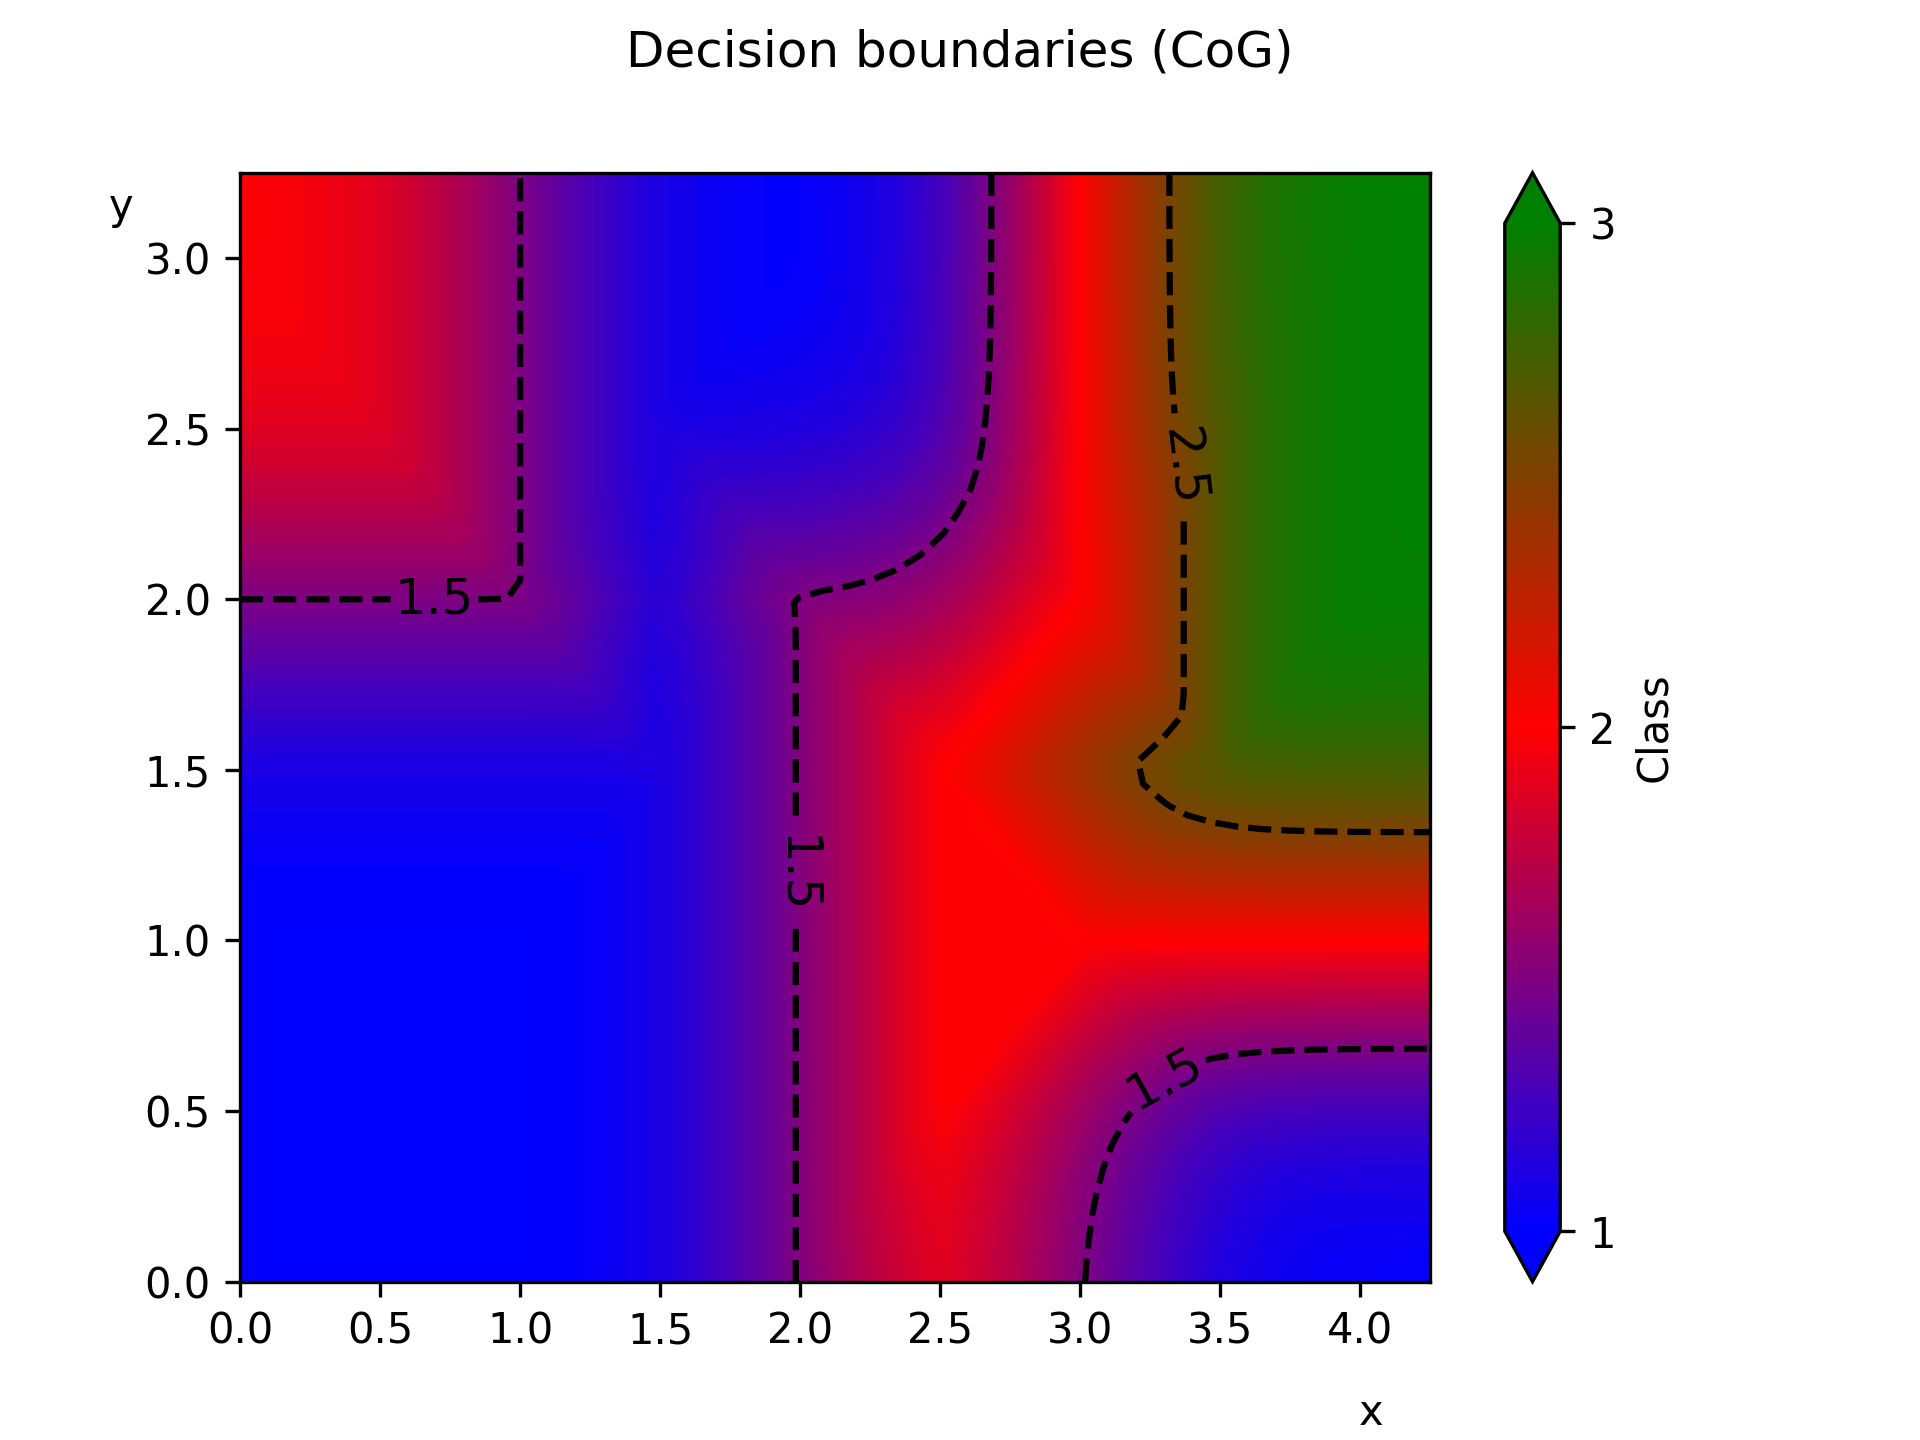
\includegraphics[width=0.9\columnwidth,trim={0 0 0 1cm},clip]{figures/ProofOfConcepts/fuzzy_system_cog.png}};
            \begin{scope}[x={(image.south east)},y={(image.north west)}]
                \draw[yellow, thin,rounded corners] (.55,.67) rectangle (.65,.95);
                \draw[yellow, thin,rounded corners] (.6,.32) rectangle (.74,.48);
                \node (A) at (.55,.56) [yellow, anchor=east] {\tiny{Interpolation Error}};

                \draw[yellow, arrow] (A) -- (.55,.67);
                \draw[yellow, arrow] (A) -- (.6,.48);
            \end{scope}
        \end{tikzpicture}

        \caption[Decision surface of the fuzzy rules using COG method]{The decision surface of the \gls{fis} created from the fuzzy decision tree in \autoref{fig:fuzzyDecisionTreeExample} over $\mathcal{D}=[0,4]\times[0,3]$ using the \gls{cog} defuzzification method. The highlighted area shows the interpolation error of the \gls{cog} method described in \autoref{fig:fuzzySetForDataCOG}.}
        \label{fig:fuzzyDecisionSurfaceExampleCOG}
    \end{figure}

    \columnbreak

    \begin{figure}[H]
        \begin{tikzpicture}
            \node[anchor=south west,inner sep=0] (image) at (0,0) { 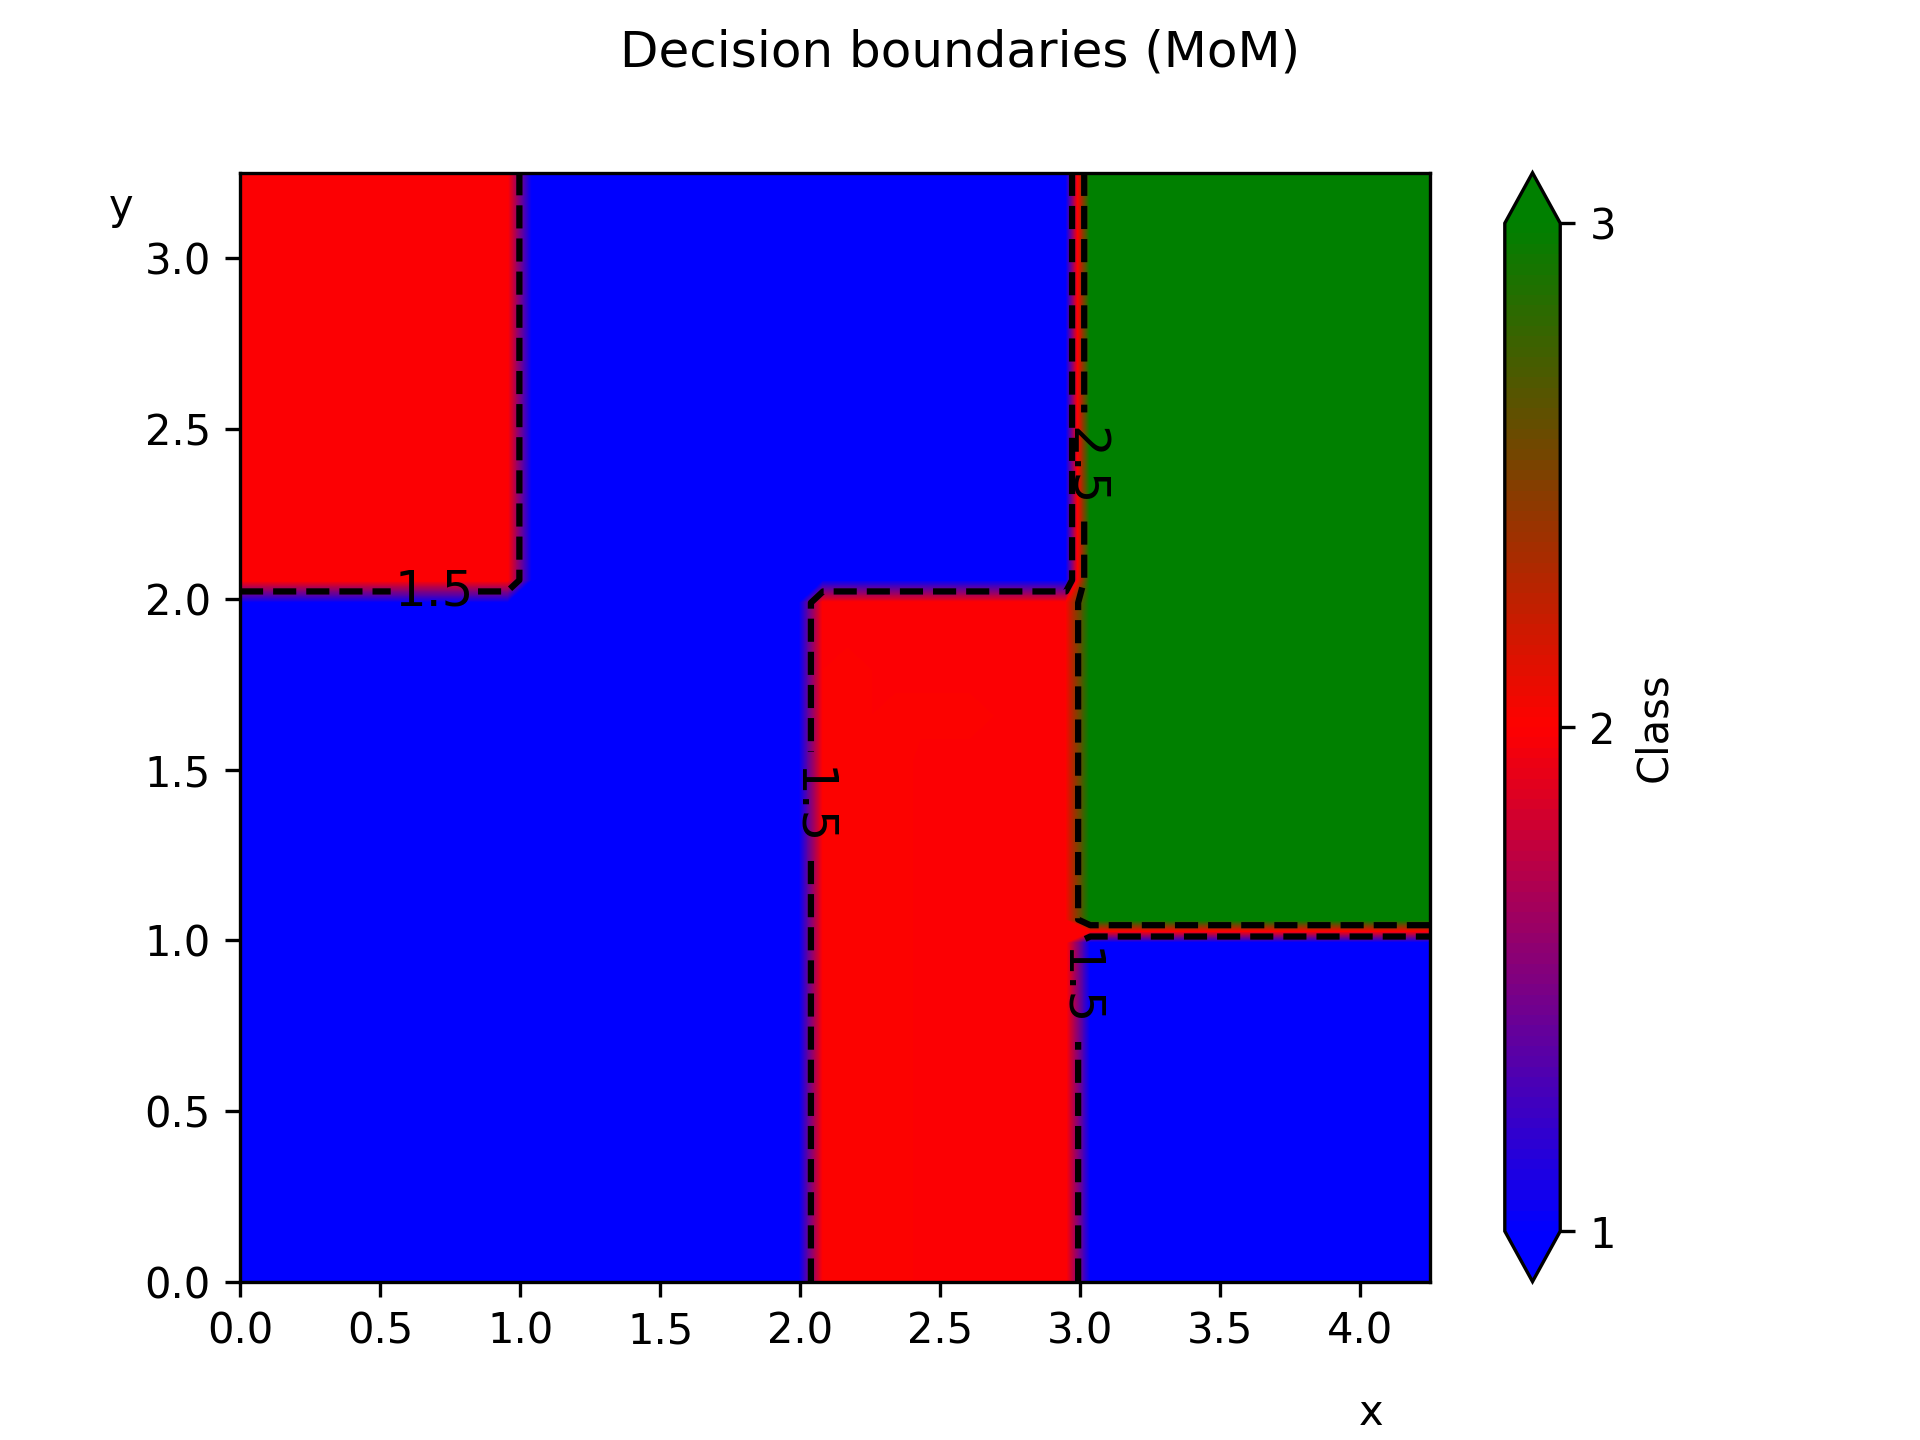
\includegraphics[width=0.9\columnwidth,trim={0 0 0 1cm},clip]{figures/ProofOfConcepts/fuzzy_system_mom.png}};
        \end{tikzpicture}
        \caption[Decision surface of the fuzzy rules using MOM method]{The decision surface of the  \gls{fis} created from the fuzzy decision tree in \autoref{fig:fuzzyDecisionTreeExample} over $\mathcal{D}=[0,4]\times[0,3]$ using the \gls{mom} defuzzification method.}
        \label{fig:fuzzyDecisionSurfaceExampleMOM}
    \end{figure}
\end{multicols}

\noindent The choice of the defuzzification method also marks the end of the conversion process, since we now have a complete fuzzy system that can be used to predict new data points based on their features. In the next section, we use this approach to create a fuzzy system to predict optimal configuration parameters for \texttt{\gls{mdflexible}} simulations.

\section{Creating a Fuzzy System for \texttt{\gls{mdflexible}}}

By following the fuzzy decision tree approach from the previous sections, we can create a fuzzy system to predict optimal configuration parameters for \texttt{\gls{mdflexible}} simulations. Contrary to the previous example, we must first collect a dataset of simulation runs with different configuration parameters and their corresponding performance metrics which can then be used to train the crisp decision tree. After the conversion of the crisp decision tree to a \gls{fis}, a human expert can evaluate the rules and membership functions and adjust them if necessary.

The resulting fuzzy system can then be used to predict the optimal configuration parameters for new simulation runs based on the current state of the simulation.

\subsection{Data Collection}

Using the \texttt{LiveInfoLogger} and \texttt{TuningDataLogger} classes of the \gls{autopas} framework, it is possible to collect all the necessary data needed to train the decision tree. Both loggers create a \texttt{.csv} file containing the simulation parameters and current runtime results for each tuning step. The \texttt{LiveInfoLogger} logs summary statistics about the simulation state such as the average number of particles per cell or the current homogeneity-estimation of the simulation, while the \texttt{TuningDataLogger} logs the current configuration and the time it took to execute the last tuning step. The full list of currently available parameters and their descriptions can be found in \autoref{des:liveinfodatafields} and \autoref{des:tuningdatafields} respectively.

We will only make use of a subset however as we are only interesed in \emph{relative} values, that don't change when the simulation is scaled up or down and are therefore only include:  \texttt{avgParticlesPerCell}, \texttt{maxParticlesPerCell}, \texttt{homogeneity}, texttt{maxDensity}, \texttt{particlesPerCellStdDev} and \texttt{threadCount}.

All the values were collected with the \texttt{PAUSE\_SIMULATION\_DURING\_TUNING} cmake option enabled, to ensure that the simulation state does not change during the tuning process. This ensures a fair comparison of the different configurations as all of them are evaluated under the same conditions.

The data was collected on the CoolMUC-2 \todo{add specs} and primarly stems from the example scenarios provided by \gls{mdflexible} such as \texttt{explodingLiquid.yaml}, \texttt{fallingDrop.yaml}, \texttt{SpinodalDecomposition.yaml} and some simulations of uniform cubes with different particle counts and densities. The exact scenarios files used for the simulations can be found in \autoref{des:scenarios}.
All simulations were run on the Serial-Partition of the the cluster were repeated twice, to account for fluctuations in performance. Furthermore every simulation was run with 1, 4, 12, 24 and 28 threads to also gather data on how parallelization affects the ideal configuration.

\subsection{Data Analysis}


To verify the sanity of the collected data, we can make plots about the distribution of the data and the nominal values of the collected data. The boxplot in \autoref{fig:inputAnalysisBoxplot} shows the distribution of the collected data, while the pie charts in \autoref{fig:inputAnalysisPiChart} shows the relative proportions of the collected parameters. We can see that the data is quite balanced and that the nominal values are spread out quite evenly, which is a good sign for the quality of the collected data.


\begin{figure}[H]
    \centering
    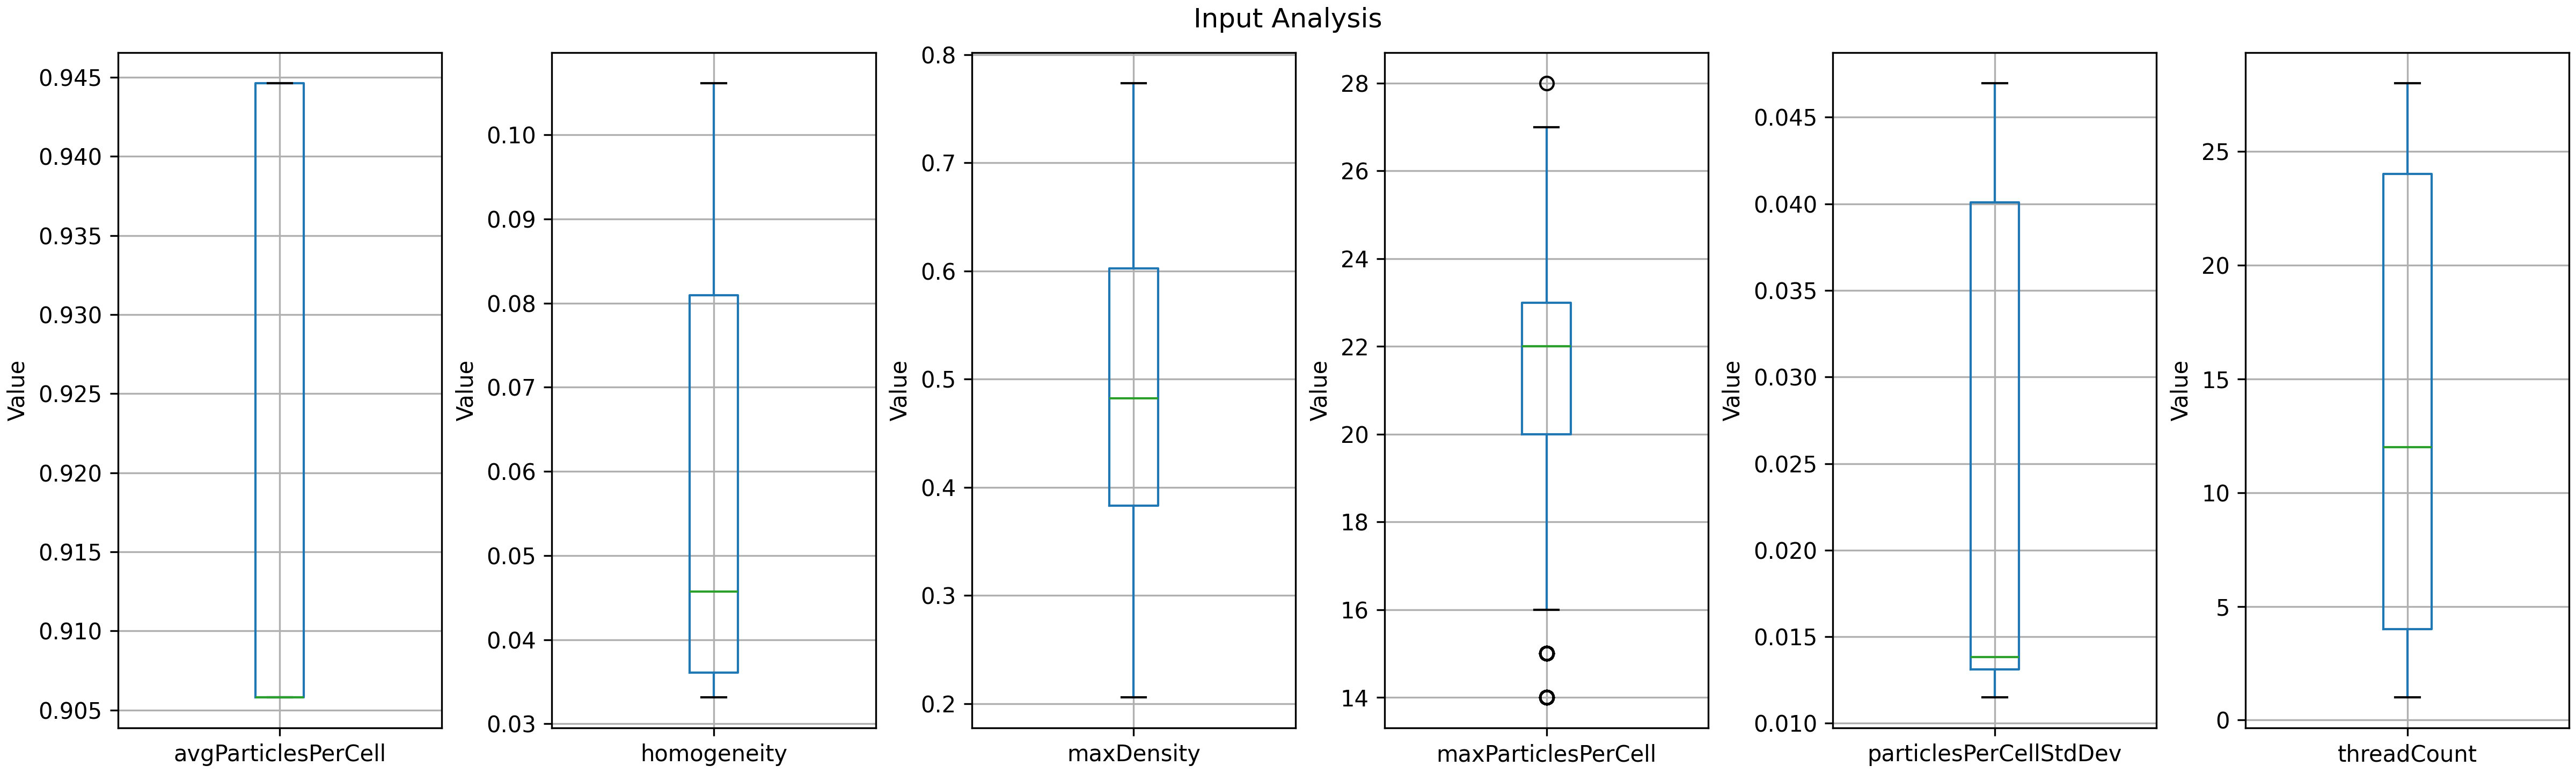
\includegraphics[width=\columnwidth,trim={0 0 0 0.5cm},clip]{figures/DataAnalytics/input_analysis.png}
    \caption[Boxplot of the collected Dataset]{The boxplot shows the distribution of the collected data. The boxplot shows the median, the first and third quartile, and the whiskers show the range of the data.}

    \label{fig:inputAnalysisBoxplot}
\end{figure}

\begin{figure}[H]
    \centering
    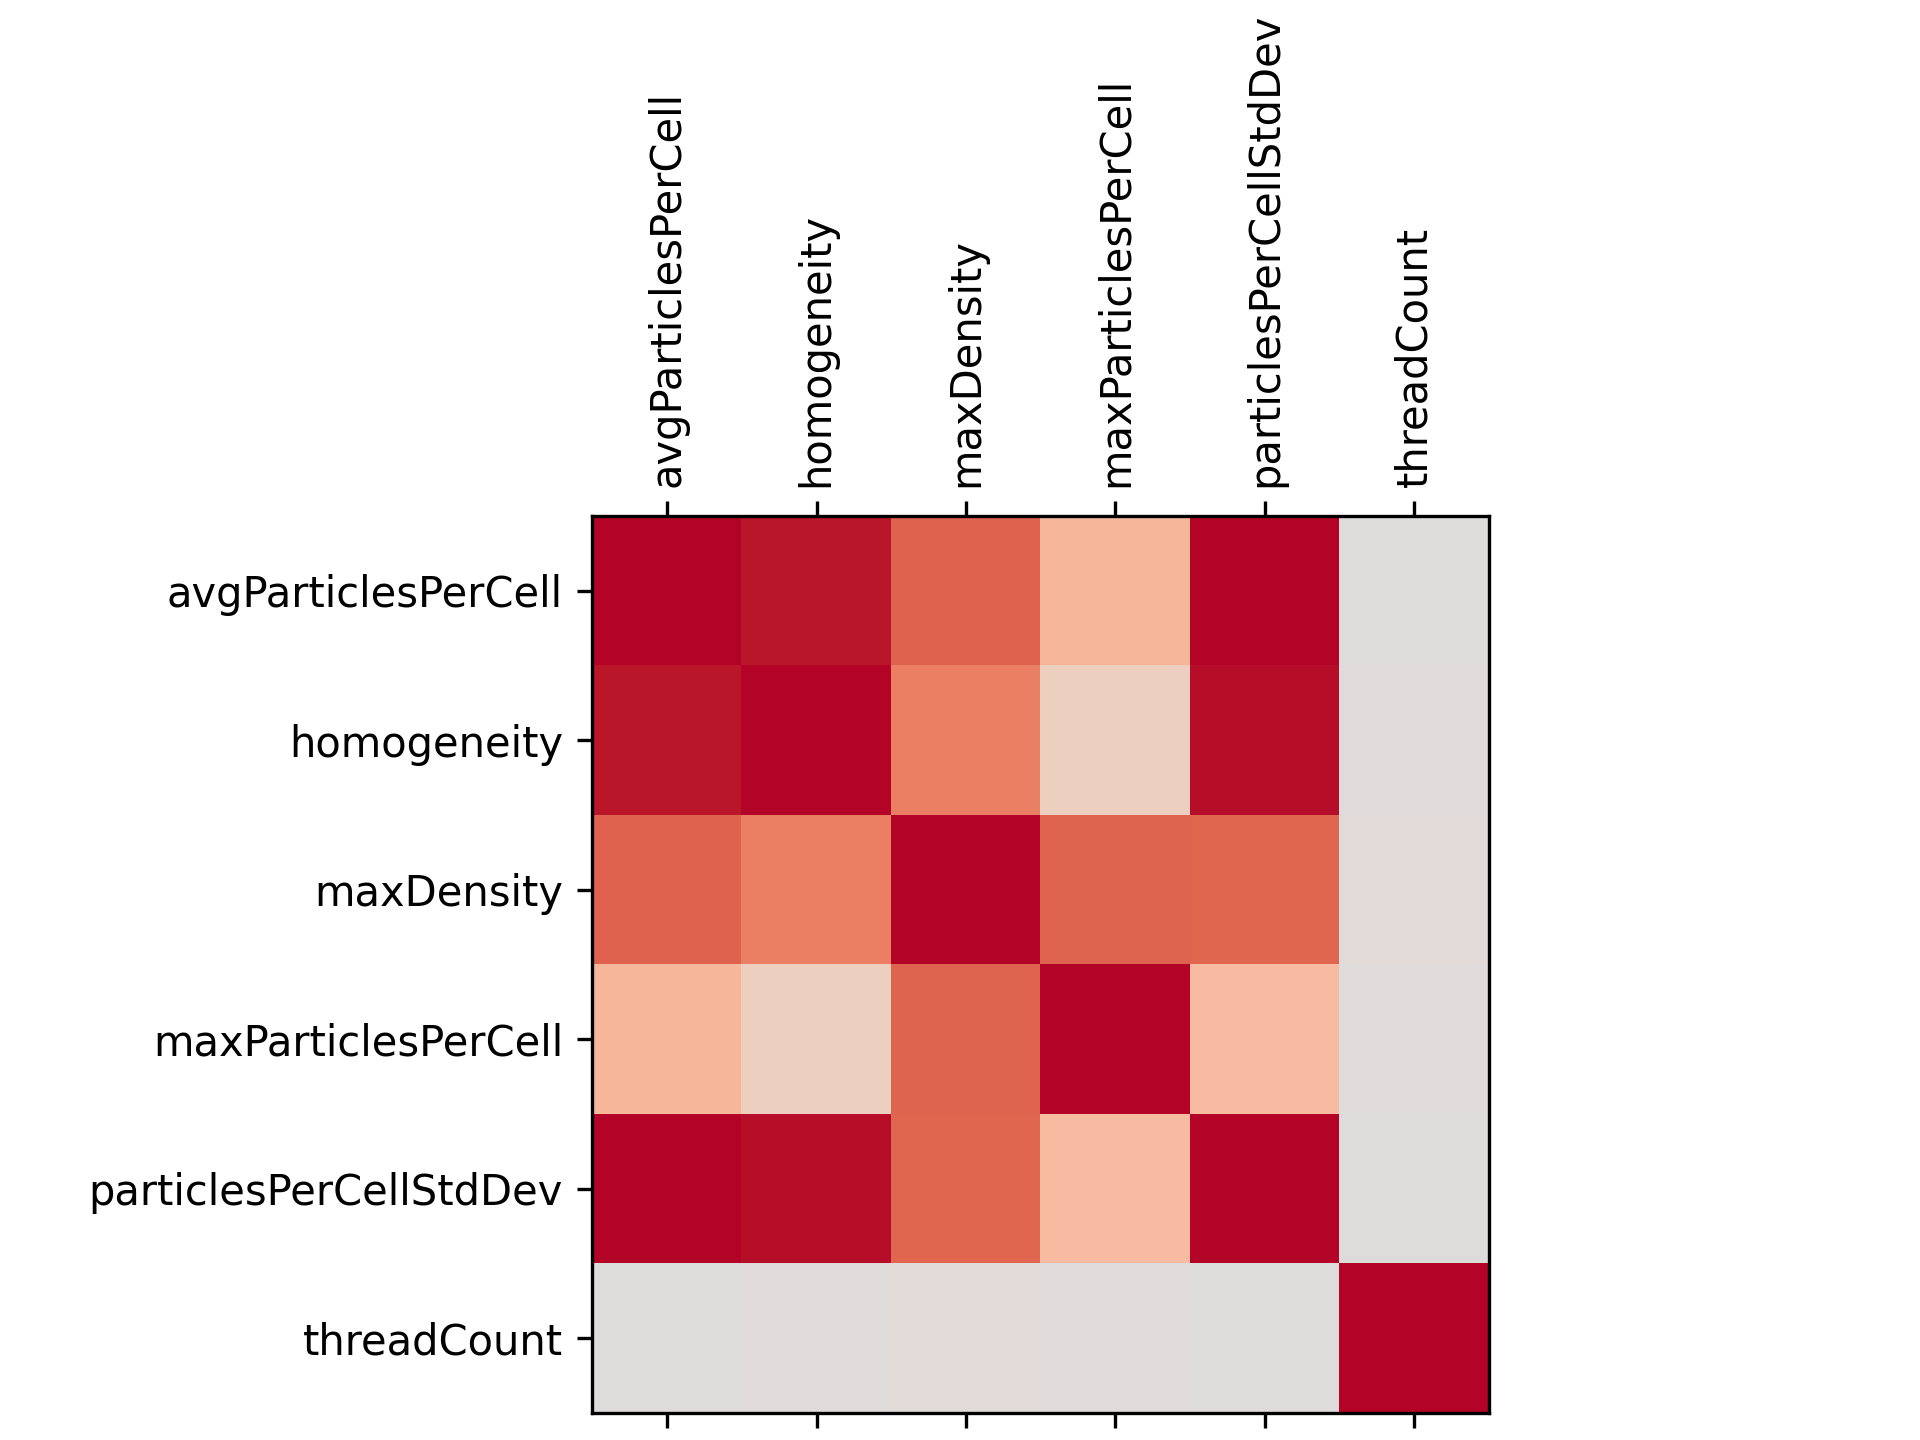
\includegraphics[height=5cm,trim={0cm 0 2cm 0cm},clip]{figures/DataAnalytics/correlation_matrix.png}
    \caption[Correlation Matrix of the collected Dataset]{The correlation matrix shows the correlation between the different parameters of the collected dataset. We can see many of the collected parameters are slighly positively correlated with each other. \texttt{particlesPerCellStdDev} is negatively correlated with \texttt{avgParticlesPerCell} and \texttt{maxParticlesPerCell} which is also expected, as a higher standard deviation of the particles per cell should lead to unbalanced cells.}
    \label{fig:corrMatrix}
\end{figure}

\begin{figure}[H]
    \centering
    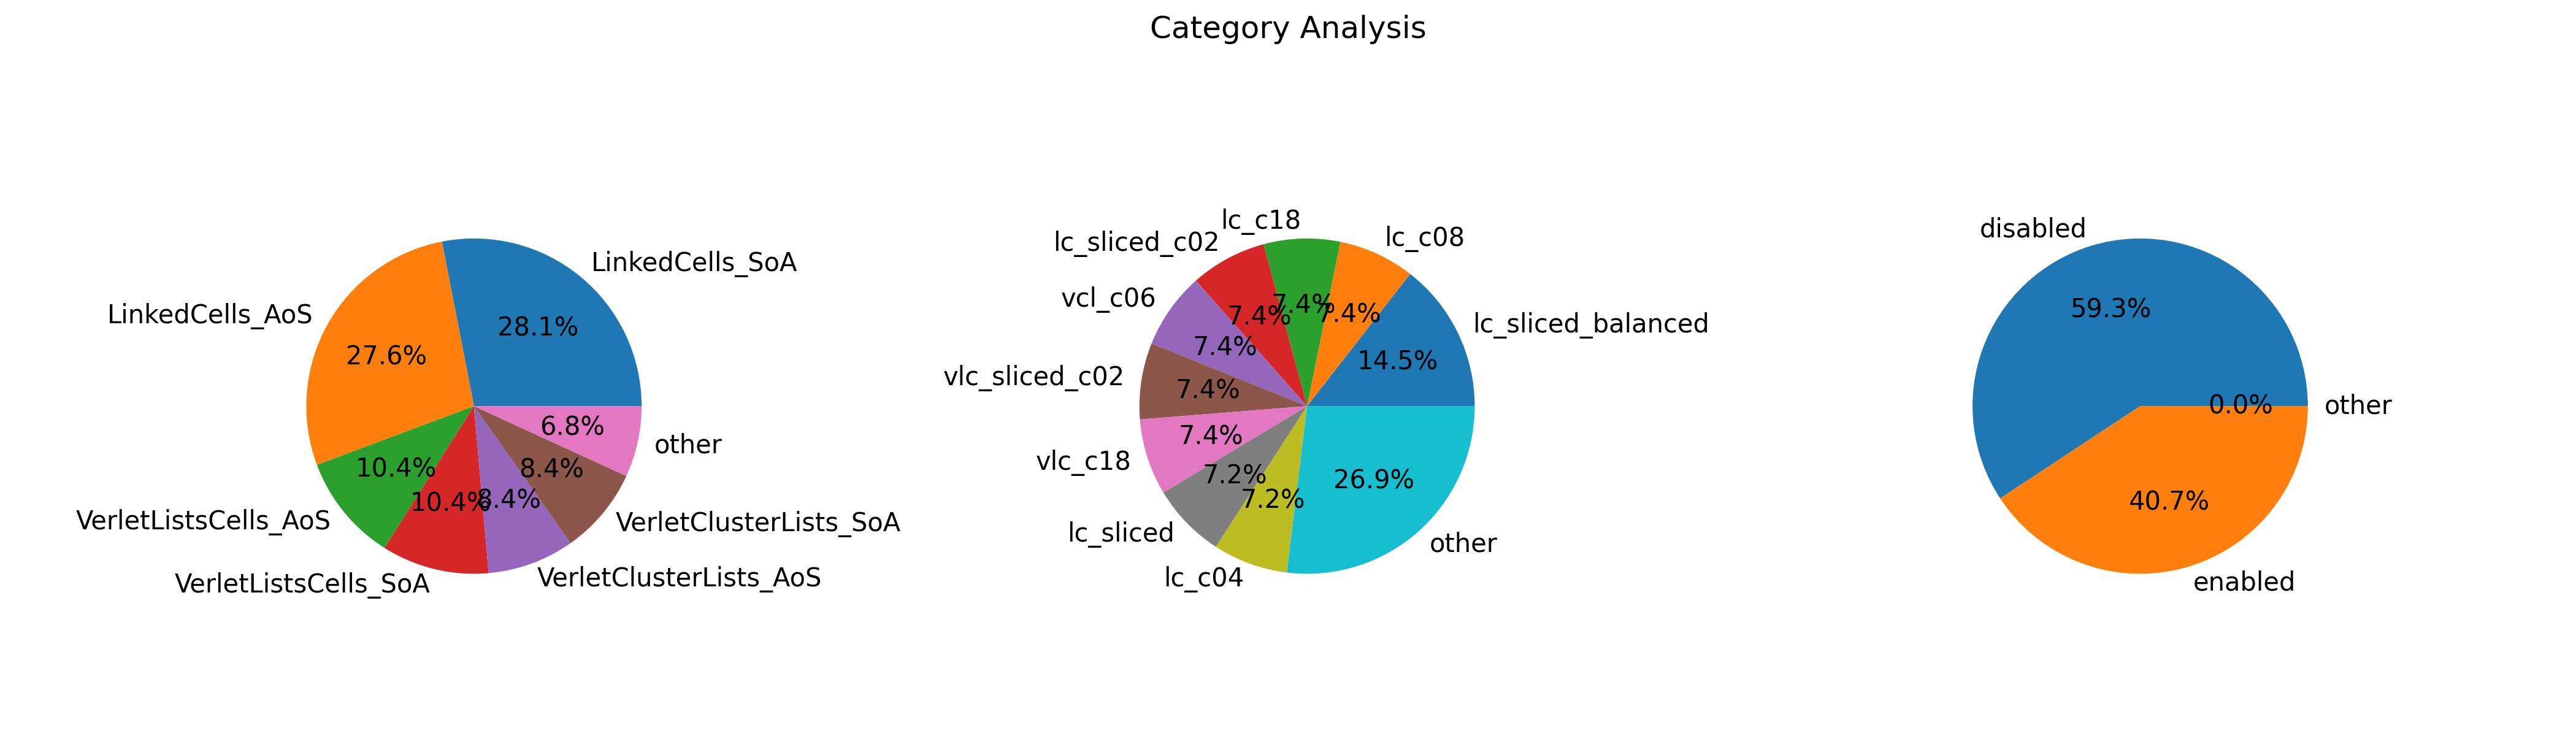
\includegraphics[width=\columnwidth,trim={1cm 2cm 2cm 2cm},clip]{figures/DataAnalytics/traversal_pie_chart.png}
    \caption[Pi Charts of nominal values of the collected Dataset]{ This figures show the relative proportions of the collected parameters in the dataset. All parameters are spread out quite evenly, which means that the dataset is quite balanced. The data however stems from every iteration, not just the tuning phases.}
    \label{fig:inputAnalysisPiChart}
\end{figure}

\subsection{Speedup Analysis}

We can also do a more detailed analysis of the average performance of the different configuration options. As we froze the simulation during the tuning process, we can safely use the runtime of each iteration as a performance metric to compare all the tested configurations. For each tuning phase there is a unique ranking of all the configurations based on their runtime which we can use to calculate the relative speedup of each configuration compared to the best configuration. The formula for the relative speedup is given by:

\begin{equation}
    {\text{speedup}^{(i)}_{\text{config}}}= \frac{t_{\text{best}}^{(i)}}{t_{\text{config}}^{(i)}}
\end{equation}

where $t_{\text{best}}^{(i)}$ is the runtime of the best configuration during the $i$-th tuning phase and $t_{\text{config}}^{(i)}$ is the runtime of the configuration we are interested in.

This means that all relative speedup values are going to be in the range $[0,1]$, with 1 being the best possible value only achieved by configurations performing optimally and 0 being the worst possible value only achieved by configurations performing \emph{infinitely} worse than the best configuration.

We can then make plots of the distribution of the relative speedup values for each configuration option to see how they affect the performance of the simulation. The density plots in \autoref{fig:inputAnalysisDensityNewton3}, \autoref{fig:inputAnalysisDensityTraversal}, \autoref{fig:inputAnalysisDensityDatalayout} and \autoref{fig:inputAnalysisDensityConfigurations} show the distribution of the relative speedup values for the Newton3, Traversal, Container-Datalayout and some complete configurations respectively. We can see that the Newton3 option generally leads to a higher relative speedup, while the Traversal option does not show a clear trend. The Datalayout option shows that the VerletListCells\_AoS option is generally the best option, while the configuration VerletListCells\_AoS\_vlc\_spliced\_balanced\_enabled is the best configuration in most cases on the Dataset we collected.

The ordering of the different parameters in the dataset matches the intuition we have about the different implementations and we can be confidently proceed with the creation of the fuzzy system.

\begin{figure}[H]
    \centering
    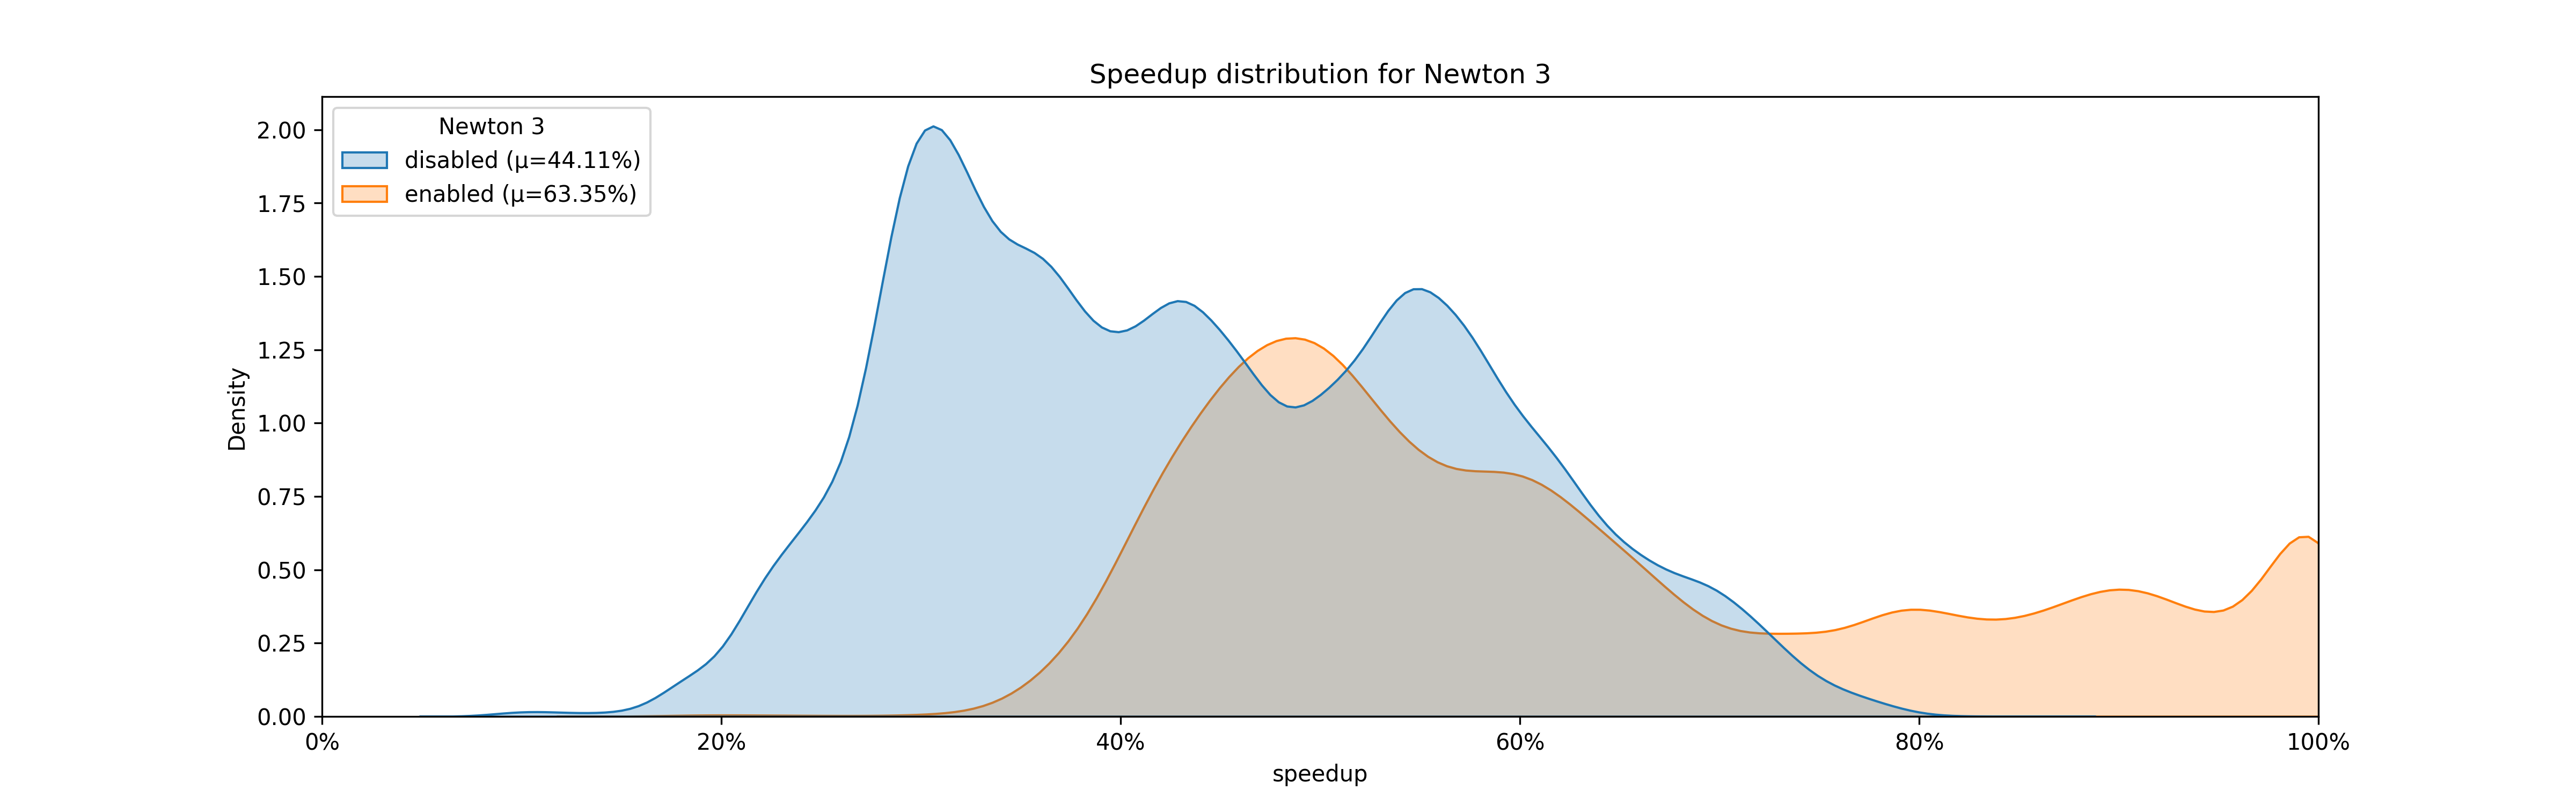
\includegraphics[width=\columnwidth,trim={1cm 0 2cm 1.5cm},clip]{figures/DataAnalytics/speedup_Newton 3.png}
    \caption[Speedup density plot of Newton 3 option]{Density plot showing the distribution of the Newton3 options with respect to their relative speedup compared to the best configuration during each tuning phase. We can clearly see the two peaks wheter Newton3 is enabled or disabled. It is also very obvious that Newton3=enabled is the better option as it generally allows for a higher relative speedup. It is interesting to note that all performances having relative speedups of at least 80\% make use of the Newton3 optimization. Therefore we can confirm that Newton3 is generally a good option to enable.}
    \label{fig:inputAnalysisDensityNewton3}
\end{figure}

\begin{figure}[H]
    \centering
    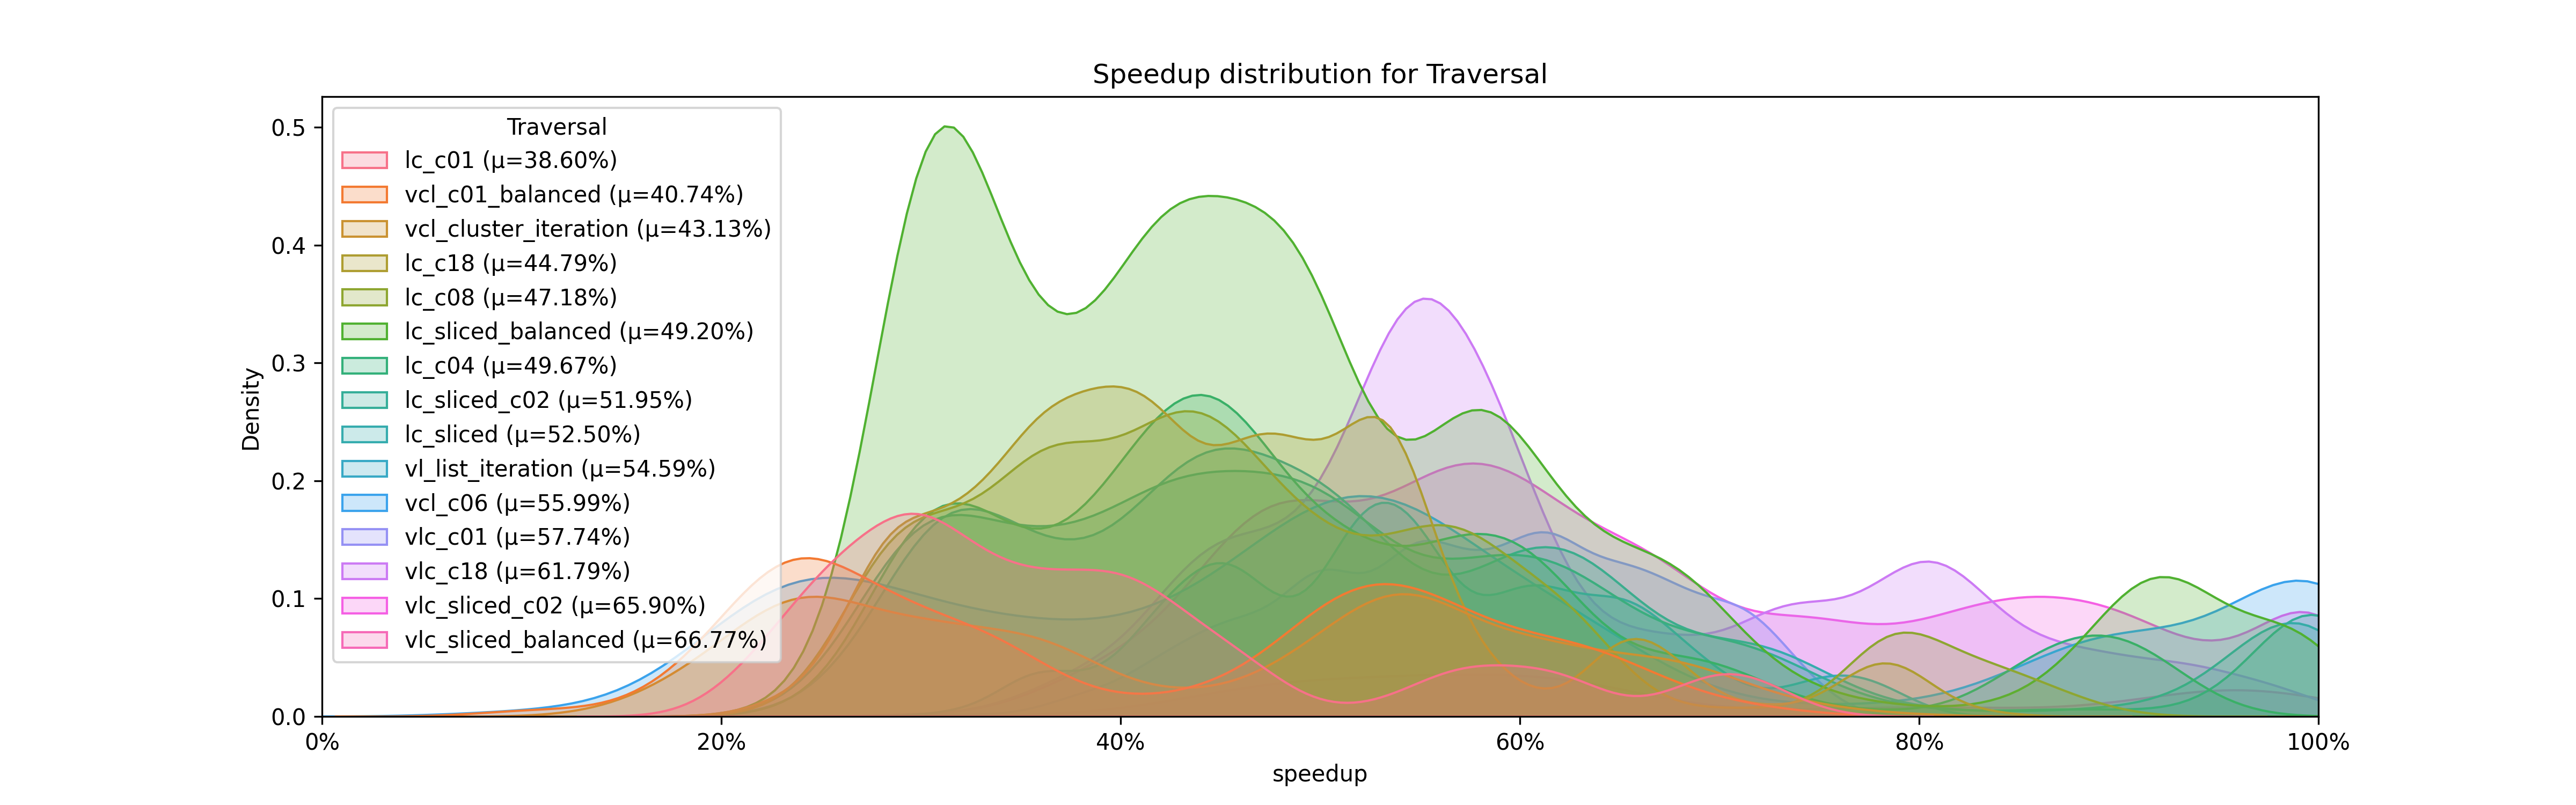
\includegraphics[width=\columnwidth,trim={1cm 0 2cm 1.5cm},clip]{figures/DataAnalytics/speedup_Traversal.png}
    \caption[Speedup density plot of Traversal option]{The density plot shows the distribution of the Traversal option with respect to the relative speedup compared to the best configuration during each tuning phase. There are no clear peaks in the data, but we can see that the vlc\_sliced\_balanced option generally performed better than the other options with an expeced relative speedup of 66\% compared to the best configuration.}
    \label{fig:inputAnalysisDensityTraversal}
\end{figure}

\begin{figure}[H]
    \centering
    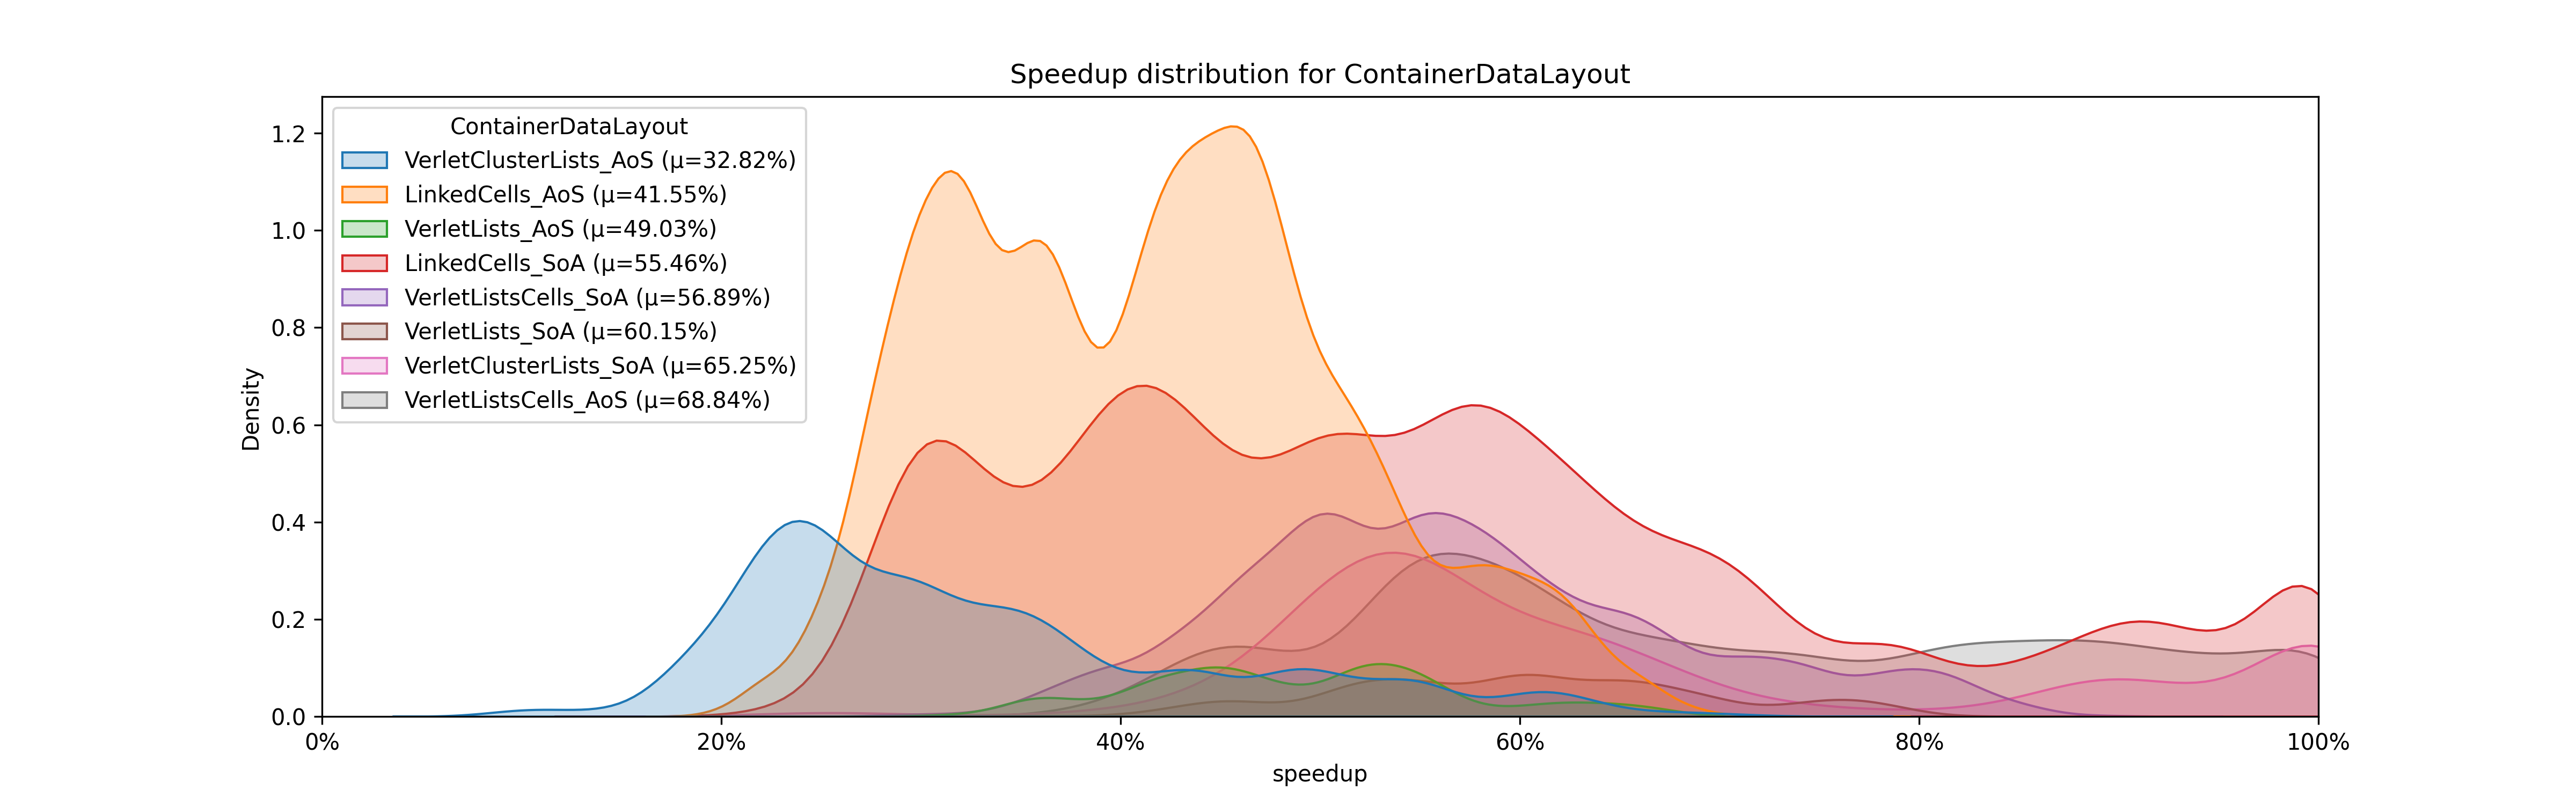
\includegraphics[width=\columnwidth,trim={1cm 0 2cm 1.5cm},clip]{figures/DataAnalytics/speedup_ContainerDataLayout.png}
    \caption[Speedup density plot of Configuration-Datalayout option]{Density plot showing the distribution of the container-datalayout option with respect to the relative speedup compared to the best configuration during each tuning phase. The VerletListCells\_AoS container-data-layout is the best configuration in most cases with 68\% of the runtime as the best configuration on average.}
    \label{fig:inputAnalysisDensityDatalayout}
\end{figure}


\begin{figure}[H]
    \centering
    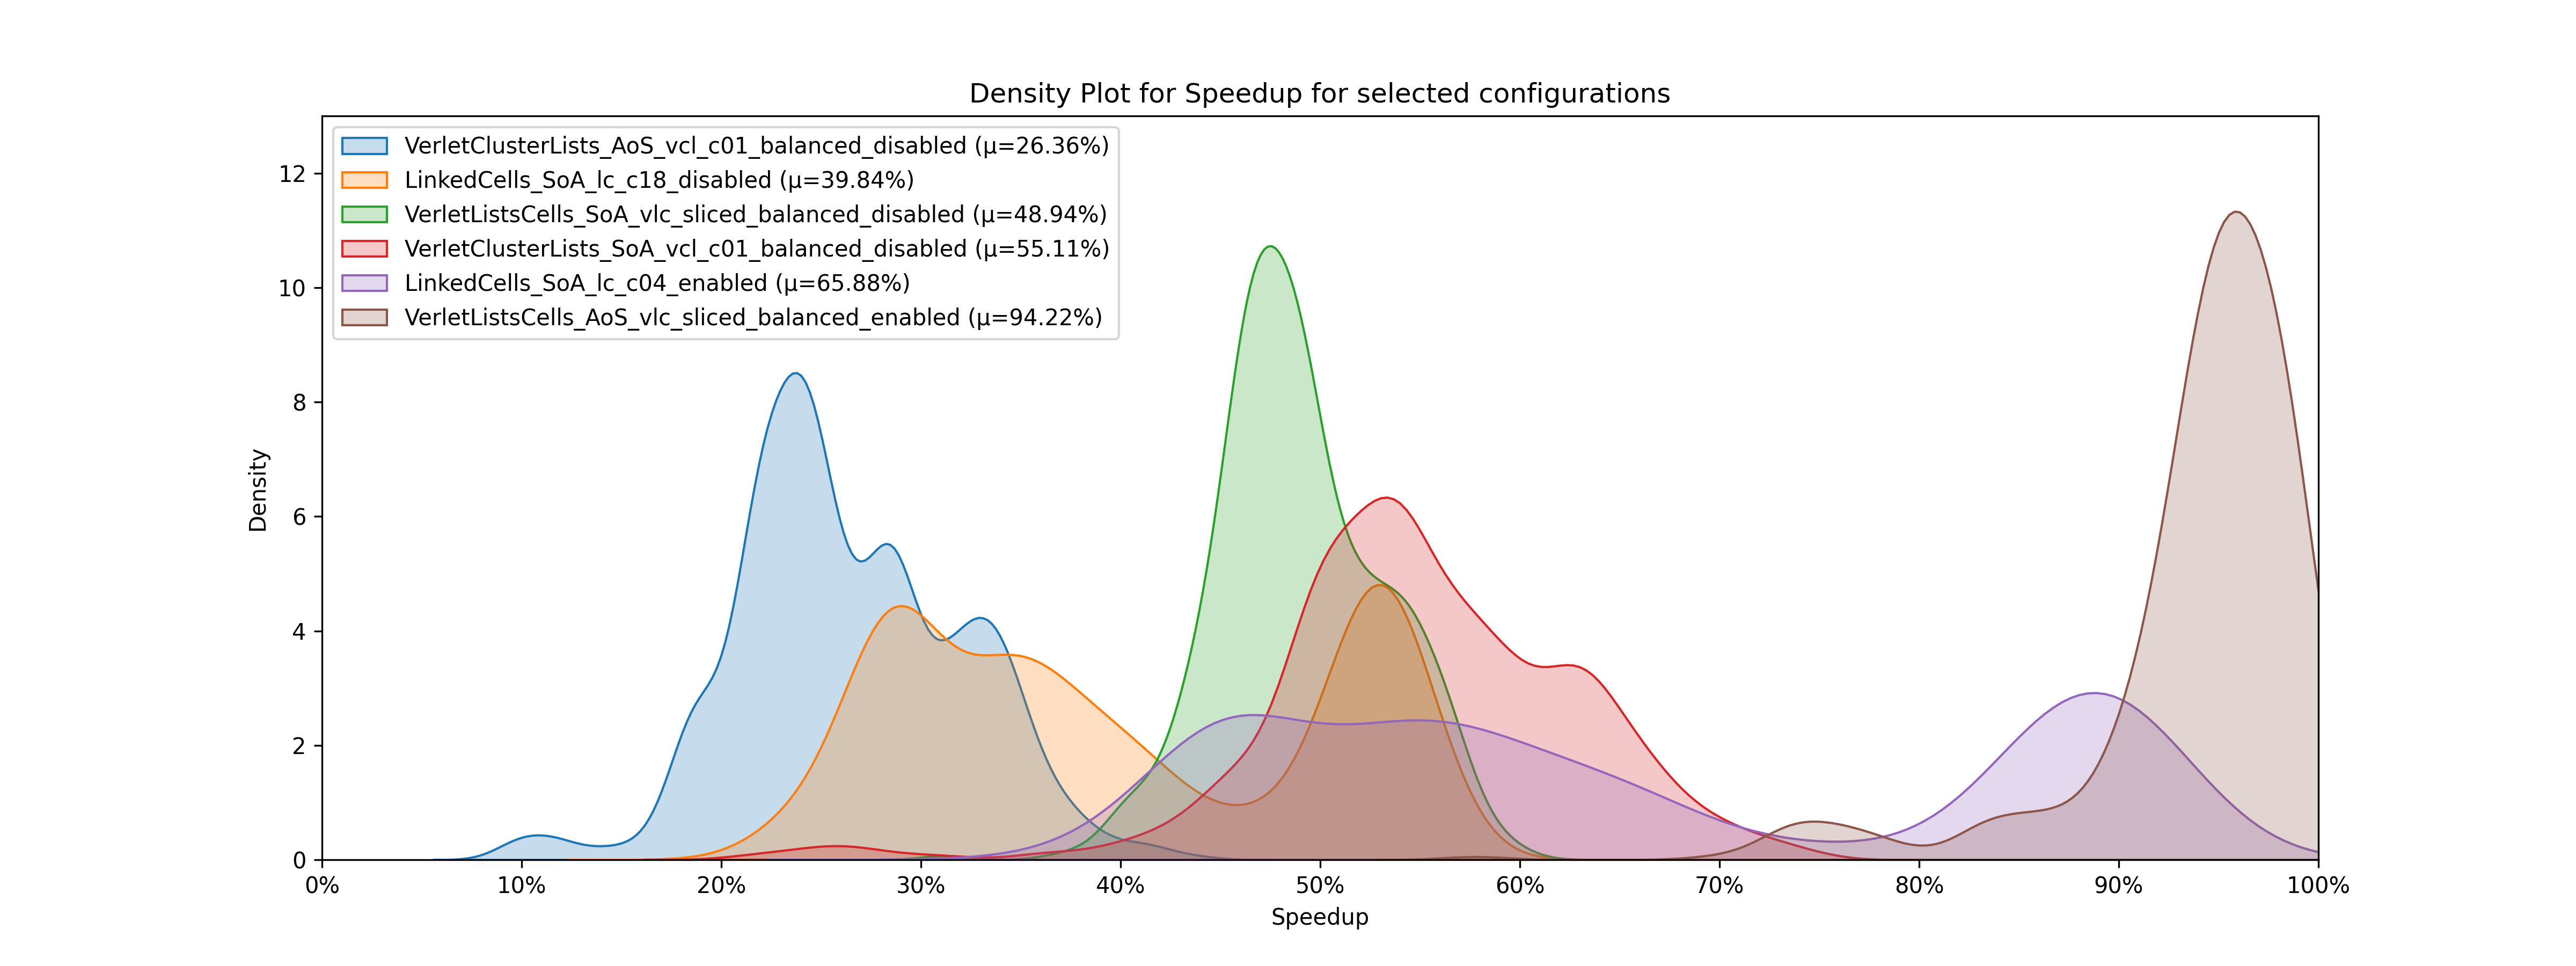
\includegraphics[width=\columnwidth,trim={1cm 0 2cm 1.5cm},clip]{figures/DataAnalytics/speedup_density_configurations.png}
    \caption[Speedup density plot of configurations]{The density plot shows the distribution of the collected configurations with respect to the relative speedup compared to the best configuration during each tuning phase. The VerletListCells\_AoS\_vlc\_spliced\_balanced\_enabled configuration is the best configuration in most cases with 94\% of the runtime as the best configuration on average.}
    \label{fig:inputAnalysisDensityConfigurations}
\end{figure}

\subsection{Creating the Fuzzy Rules}

By using the decision tree approach described in the previous sections, we can create a fully automated system to transform the collected data into rulefiles. The process is as follows:

\begin{enumerate}
    \item Preprocess the data according to to approach used (see next section).
    \item Train the decision trees and prune the tree to avoid overfitting.
    \item Select the best perfoming decision trees and convert them into fuzzy decision trees.
    \item Extract the fuzzy rules from the fuzzy decision trees.
    \item Generate the linguistic variables and terms for the fuzzy system.
    \item Create the OutputMapping Export and export everything to a rulefile.
\end{enumerate}

As described previously, we are going to create two different kind of rule-bases, one for the Suitability Approach and one for the Individual Tuning Approach. In the following sections we will describe both approaches in detail.

\subsection{Individual Tuning Approach}

This approach tries to create different fuzzy systems for each of the tunable paramters of the simulation. We decided to combine the \texttt{container} and \texttt{dataLayout} parameters into a single parameter as they are closely related and the performance of one is heavily dependent on the other. Consequently we want to create systems for \texttt{ContainerDataLayout}, \texttt{Traversal} and \texttt{Newton3}.

As we only want to create a fuzzy system predicting good configurations, we first remove all configurations perfoming worse than a certain threshold. As depicted in \autoref{fig:speedup} we chose to only include configurations that have a relative speedup of at least 70\% as this still leaves us with a large enough dataset to train the decision trees.

\begin{figure}[H]
    \centering
    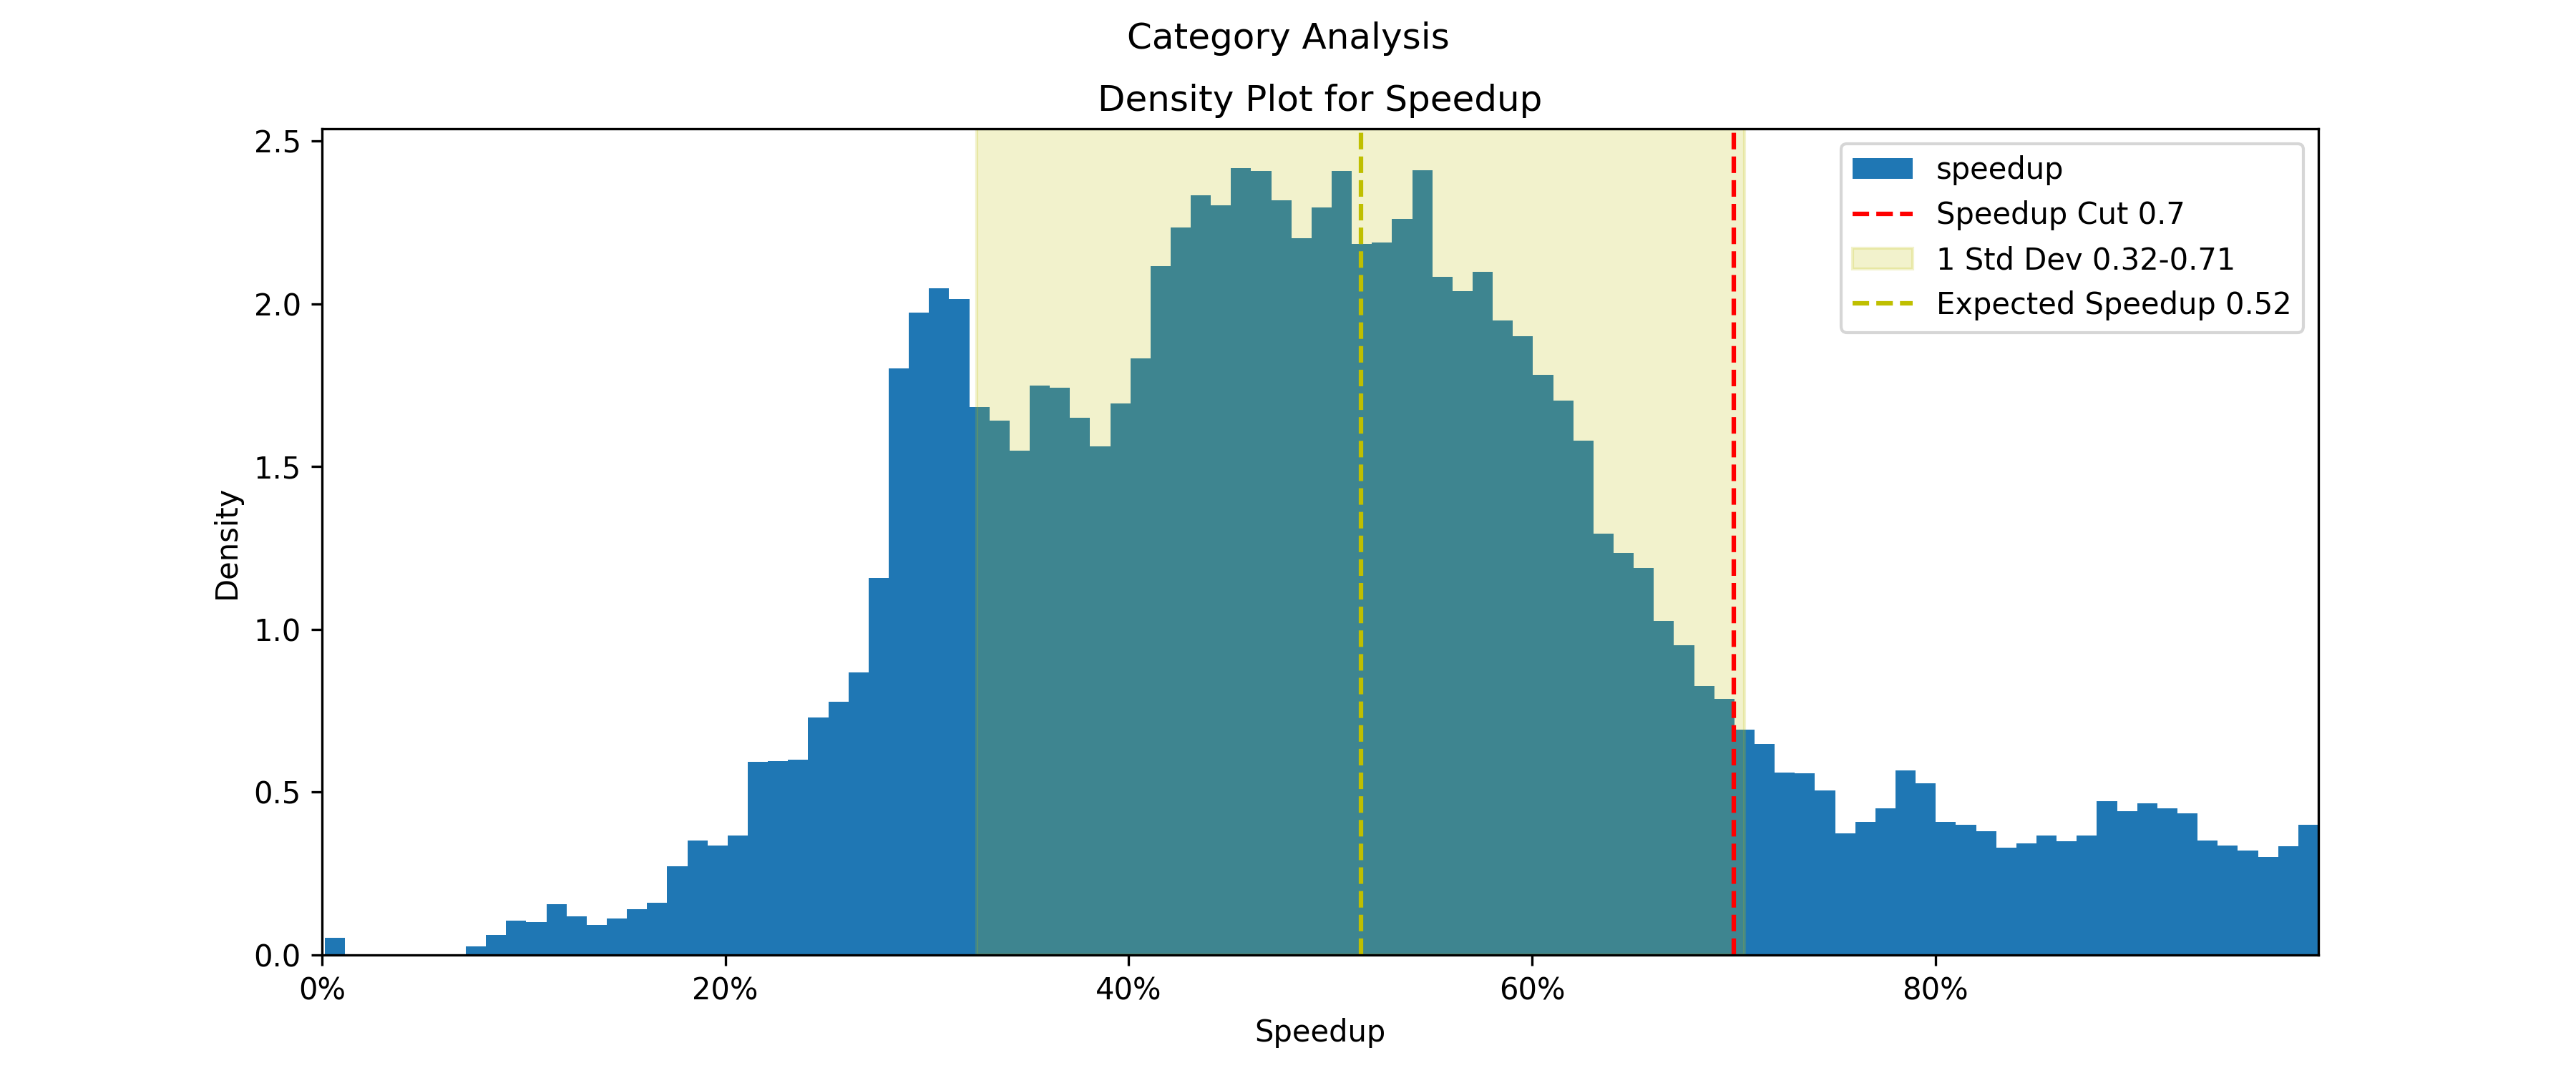
\includegraphics[width=\columnwidth,trim={1cm 0 2cm 1.5cm},clip]{figures/DataAnalytics/speedup.png}
    \caption[Speedup density plot of all configurations]{The density plot shows the distribution of all the collected configurations with respect to the relative speedup compared to the best configuration during each tuning phase. This distribution shows that the average tested configuration performs just 50\% as good as the best. With some configurations beeing 10 times slower than the best configuration.
        We see that it is of utmost importance to efficiently find good configurations as testing all possible configurations causes a huge performance loss.}
    \label{fig:speedup}
\end{figure}

Afterward we group together all configurations that have been evaluated in the same tuning phase and aggregate all the present values of tunable parameters into a single term. This term representing all \emph{good} values for the paramters to be chosen under the conditions of the tuning phase. The resulting training data is shown in \autoref{tab:trainingDataIndividual} and can be used to train the decision trees. After applying the transformation process described in the previous sections, we end up with rules shown in \autoref{tab:fuzzyRulesIndividual}. This concludes the creation of the fuzzy rules for the Individual Tuning Approach.


\begin{table}[H]
    \footnotesize
    \centering
    \begin{tabular}{|c|c|c|c|c|}
        \hline

        \textbf{LiveInfo Data} & \textbf{Container\_DataLayout} & \textbf{Traversal} & \textbf{Newton3} \\
        \hline
        \makecell{(0.905797,	0.055112,                                                                   \\	0.297891,	15,	0.015171,	4) }                                                                                                              & \makecell{"LinkedCells\_SoA,                                                \\ VerletClusterLists\_SoA, \\ VerletListsCells\_AoS"} & \makecell{"lc\_sliced,\\ lc\_sliced\_balanced,\\ lc\_sliced\_c02,\\ lc\_c04"} & "enabled"          \\
        \hline
        \makecell{(0.944637,	0.084061,                                                                   \\	0.673320,                                                                                                                                                                                                   	25,	0.039916, 24) }                                                                                                               & \makecell{"LinkedCells\_SoA,                                                \\ VerletClusterLists\_SoA, \\ VerletListsCells\_AoS"} & \makecell{"lc\_c04,\\ lc\_c08,\\ lc\_sliced,\\ lc\_sliced\_balanced"} &  \makecell{"disabled,\\enabled"}         \\
        \hline
        \makecell{(0.905797,	0.041394,                                                                   \\	0.336900,                                                                                                                                                                                                   	20,	0.013546, 24) }                                                                                                               & \makecell{"VerletClusterLists\_SoA,                                         \\ VerletListsCells\_AoS"} & \makecell{"vcl\_c06,\\ vlc\_c01,\\ vlc\_c18,\\ vlc\_sliced\_c02"} &  \makecell{"disabled,\\enabled"}         \\
        \hline

        \vdots                 & \vdots                         & \vdots             & \vdots           \\
        \hline
    \end{tabular}
    \caption[Prepared training data for the Individual Tuning Approach]{Selection of the prepared training data for the Individual Tuning Approach. The table shows the liveinfo data and the corresponding prediction of top performing values for each tunable parameter. Each row represents a different tuning phase.}
    \label{tab:trainingDataIndividual}
\end{table}




\definecolor{LightCyan}{rgb}{0.88,1,1}
\newcolumntype{g}{>{\columncolor{LightCyan}}c}

\begin{table}[H]
    \footnotesize
    \centering
    \addtolength{\leftskip} {-3cm} % increase (absolute) value if needed
    \addtolength{\rightskip}{-3cm}

    \begin{tabular}{|c|c|c|c|g|}
        \multicolumn{4}{c}{\large{\textbf{Antecedent}}} & \multicolumn{1}{c}{\large{\textbf{Consequent}    }}                                                                                                                                    \\
        \hline
        \textbf{avgParticlesPC}                         & \textbf{homogeneity}                                & \textbf{particlesPCStdDev}                        & \textbf{threadCount}      & \textbf{ContainerDataLayout}                     \\

        \hline
        \texttt{lower than 3.454}                       & \texttt{lower than 0.05}                            &                                                   & \texttt{lower than 18.0}  & \tabularCenterstack{c}{"VerletClusterLists\_SoA, \\
        VerletListsCells\_AoS"}                                                                                                                                                                                                                  \\
        \hline
        \texttt{lower than 3.454}                       & \texttt{higher than 0.05}                           & \texttt{lower than 0.024}                         & \texttt{higher than 18.0} & \tabularCenterstack{c}{"LinkedCells\_SoA,        \\ VerletClusterLists\_SoA,\\ VerletListsCells\_AoS"}  \\
        \hline
        \vdots                                          & \vdots                                              & \vdots                                            & \vdots                    & \vdots                                           \\
        \hline

        \multicolumn{5}{c}{ }                                                                                                                                                                                                                    \\


        \multicolumn{4}{c}{\large{\textbf{Antecedent}}} & \multicolumn{1}{c}{\large{\textbf{Consequent}    }}                                                                                                                                    \\

        \hline
        \textbf{avgParticlesPC}                         & \textbf{homogeneity}                                & \textbf{particlesPCStdDev}                        & \textbf{threadCount}      & \textbf{Traversal}                               \\

        \hline

        \texttt{lower than 1.553}                       & \texttt{higher than 0.047}                          & \texttt{lower than 0.023	}                         & \texttt{higher than 2.5}  & \tabularCenterstack{c}{"lc\_sliced,              \\ vlc\_c18,\\ lc\_sliced\_c02"}
        \\
        \hline

                                                        & \texttt{lower than 0.037}                           & \texttt{lower than 0.023	}                         & \texttt{lower than 26.0}  & \tabularCenterstack{c}{"vcl\_c06,                \\ vlc\_c18,\\ vlc\_sliced\_c02"}                                                          \\


        \hline
        \vdots                                          & \vdots                                              & \vdots                                            & \vdots                    & \vdots                                           \\
        \hline


        \multicolumn{5}{c}{ }                                                                                                                                                                                                                    \\


        \multicolumn{4}{c}{\large{\textbf{Antecedent}}} & \multicolumn{1}{c}{\large{\textbf{Consequent}    }}                                                                                                                                    \\

        \hline
        \textbf{avgParticlesPC}                         & \textbf{homogeneity}                                & \textbf{particlesPCStdDev}                        & \textbf{threadCount}      & \textbf{Newton 3}                                \\

        \hline

                                                        &                                                     & \texttt{higher than 0.03}                         & \texttt{higher than 18.0} & \tabularCenterstack{c}{"disabled,                \\enabled"}
        \\
        \hline

                                                        &                                                     & \tabularCenterstack{c}{\texttt{higher than 0.023}                                                                                \\ $\land$ \texttt{lower than 0.037	}} &  \tabularCenterstack{c}{\texttt{lower than 18.0}\\ $\land$ \texttt{higher than 8.0	}} & \tabularCenterstack{c}{"enabled"}                \\


        \hline
        \vdots                                          & \vdots                                              & \vdots                                            & \vdots                    & \vdots                                           \\
        \hline
    \end{tabular}

    \caption[Extracted fuzzy rules for the Individual Tuning Approach]{Extracted fuzzy rules for the Individual Tuning Approach. The table shows a selection of the rules extracted from the decision trees trained on the training data in \autoref{tab:trainingDataIndividual}. The columns of the antecedent represent the different fuzzy sets taking part in the rule.}
    \label{tab:fuzzyRulesIndividual}
\end{table}

As descibed previously we use \texttt{gaussian} membership functions for each linguistic term of the consequent linguistic variables. The placement of the  values is irrelevant and we just place them in a way that they don't overlap. \autoref{fig:homogenityLinguisticVariable} and \autoref{fig:newton3LinguisticVariable_individual} show the resulting linguistic variables for a antecedent linguistic variable (homogeneity) and a consequent linguistic variable (Newton3) respectively. The visualization of the other variables follows a similar pattern, but are more complex due to the higher number of terms and are therefore not shown here.



\begin{multicols}{2}
    \begin{figure}[H]
        \centering
        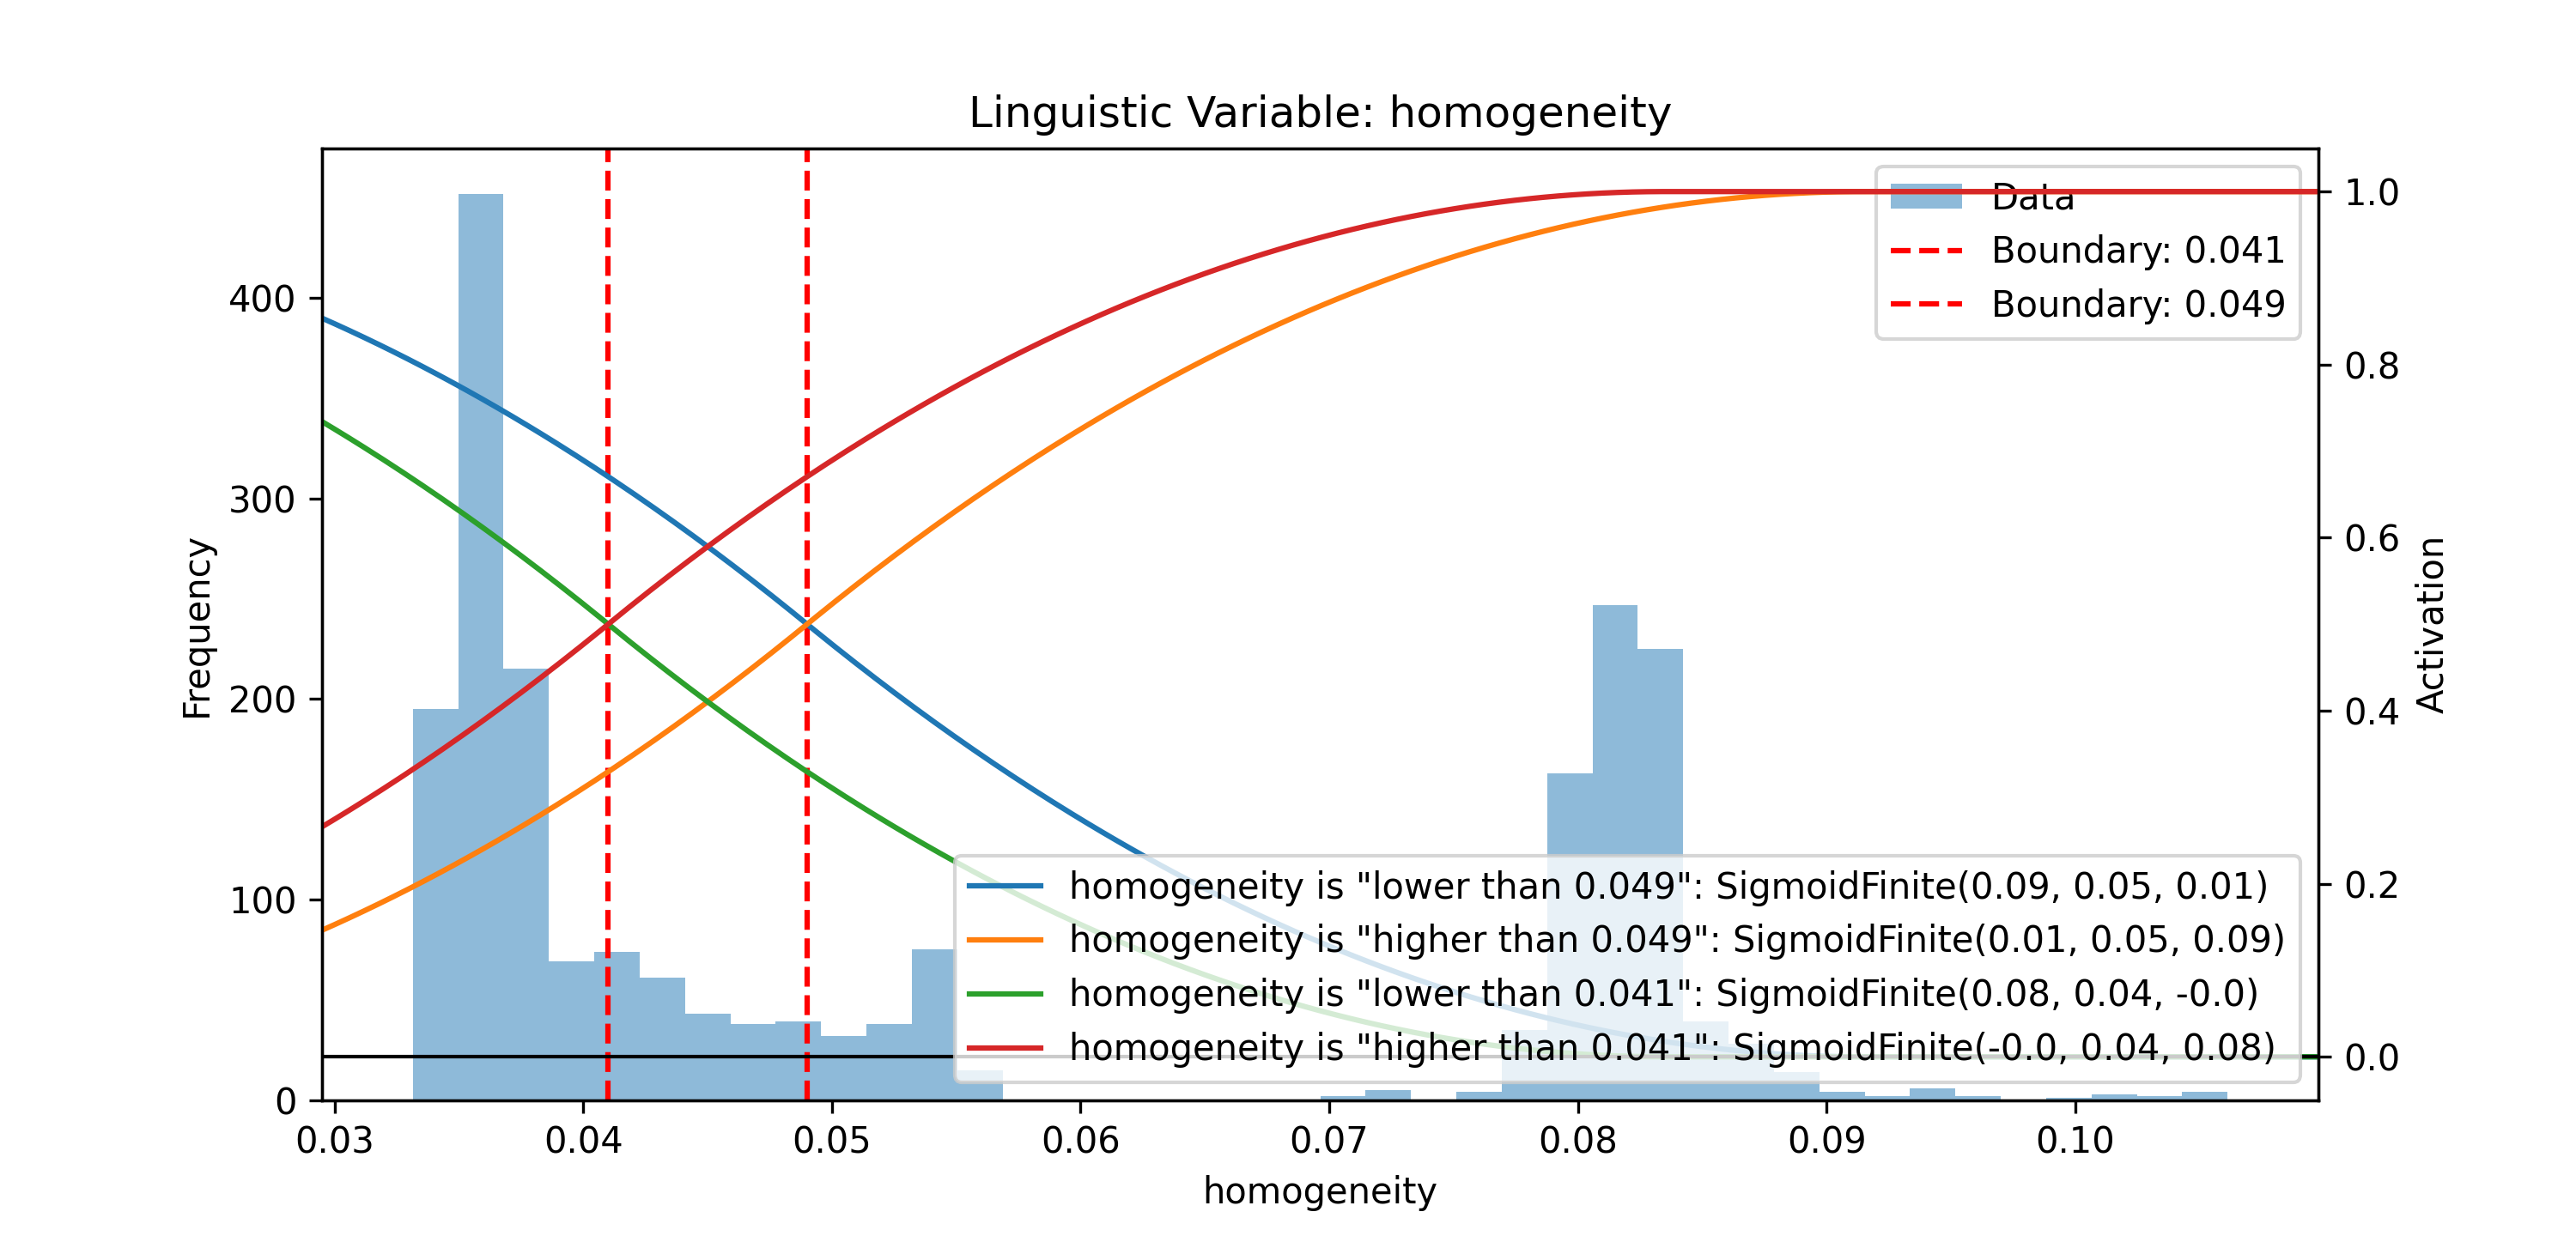
\includegraphics[width=\columnwidth,trim={1cm 0 1cm 1.35cm},clip]{figures/DataAnalytics/homogenity_linguistic_variable.png}

        \caption[Linguistic variable for the homogeneity attribute]{
            This figure shows the linguistic variable for the homogeneity attribute. We see the different fuzzy sets created from the decision trees. The background shows the histogram of all homogeneity values present in the dataset.
        }
        \label{fig:homogenityLinguisticVariable}
    \end{figure}

    \columnbreak

    \begin{figure}[H]
        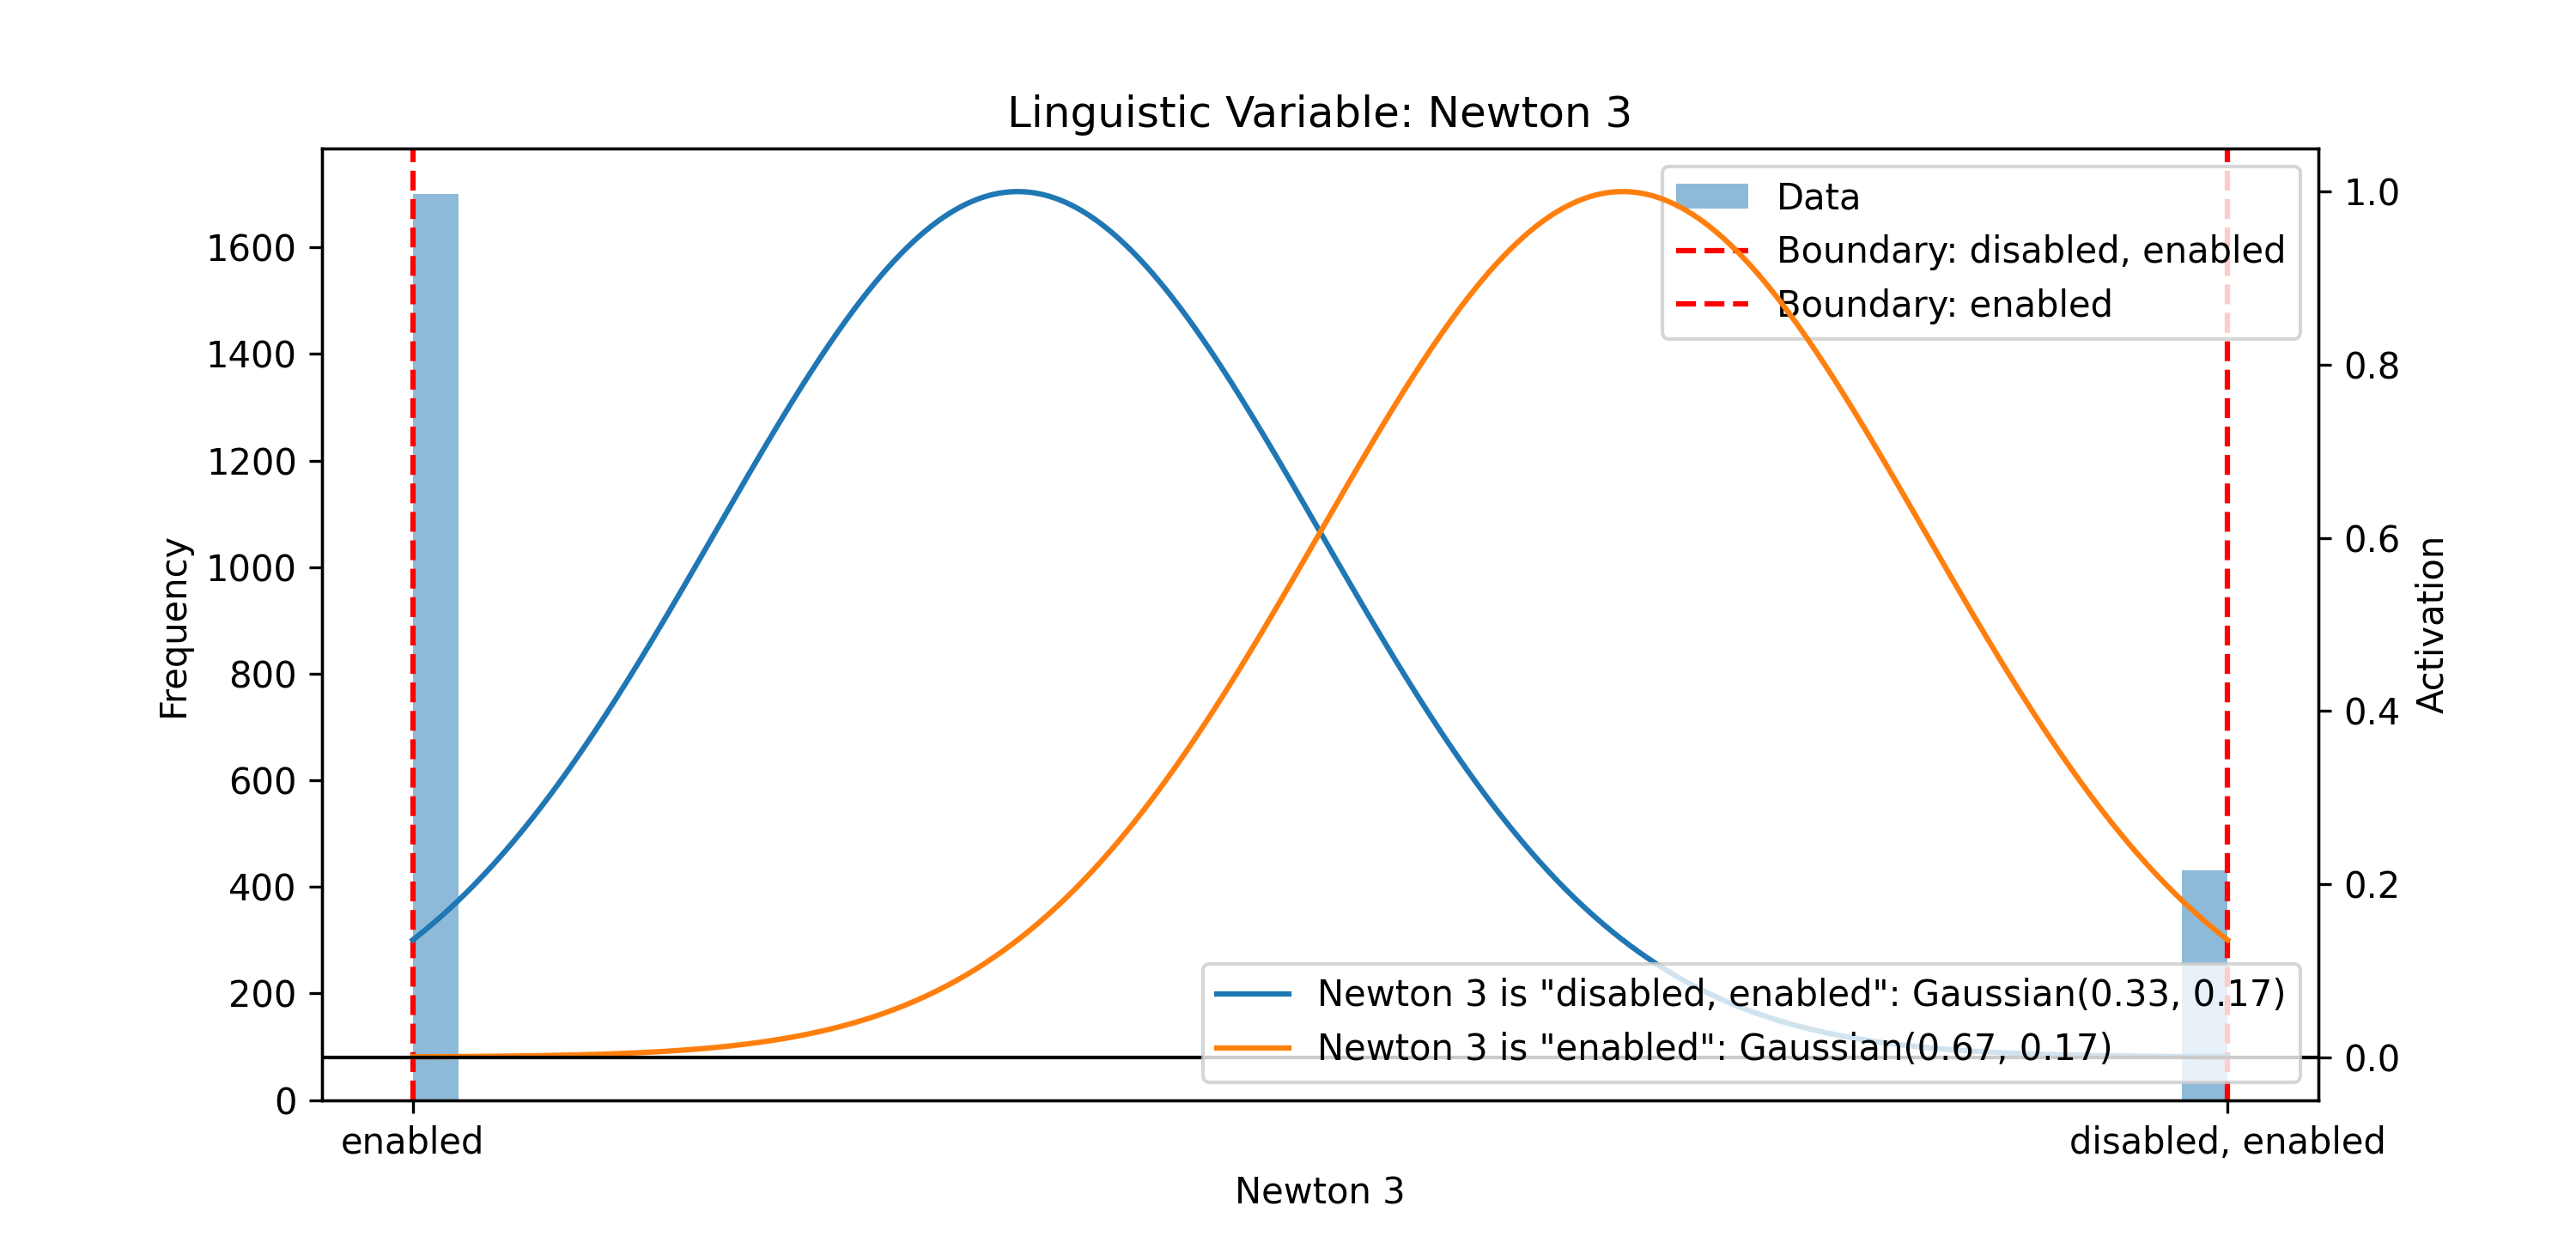
\includegraphics[width=\columnwidth,trim={1cm 0 1cm 1.35cm},clip]{figures/DataAnalytics/newton3_linguistic_variable.png}
        \caption[Linguistic variable for the Newton3 attribute]{
            This figure shows the linguistic variable for the Newton3 attribute. We see the two \texttt{gaussian} membership functions representing the two possible values for the Newton3 attribute.
        }
        \label{fig:newton3LinguisticVariable_individual}
    \end{figure}
\end{multicols}

At the end of the process we have different fuzzy systems for each of the tunable parameters of the simulation of the form shown in \autoref{fig:fuzzyInferenceSystemIndividual}. The fuzzy system can be seen as a black box that maps the LiveInfo data into a sort of \emph{index} representing the the predicted values of the parameter. As we are using the \gls{mom} method, the output will always correspond to the fuzzy set with the highest membership value and will be free of interpolation errors. Using the output mappings of the form shown in \autoref{lst:outputMappingIndividual} we can then convert the predicted \emph{index} into a format suitabile for AutoPas.

\begin{lstlisting}[language=FuzzyLanguage, caption={OutputMapping for the Individual Tuning Approach}, label={lst:outputMappingIndividual}]
    OutputMapping:
      "Newton 3":
//      index => predicted configuration values
        0.333 =>  [newton3="disabled"]
        0.666 =>  [newton3="disabled"], [newton3="enabled"]
    ...
    
\end{lstlisting}

\begin{figure}[H]
    \centering
    \begin{tikzpicture}[scale=2,font=\small]
        \node[anchor=east] (L) at (-2,0.6) {$\text{LiveInfo} \in \mathbb{R}^d$};

        \foreach \x in {5,...,1}
            {
                \node [rectangle,rounded corners,draw,inner sep=2pt,fill=white!80!black] (A) at (0+\x /5,0+\x/4) {
                    \begin{tikzpicture}[scale=2- \x/8 ,font=\tiny]
                        \begin{axis}%
                            [
                                title={FIS [paramter\textsubscript \x]},
                                width=3.2cm,
                                height=2cm,
                                axis lines=center,
                                xmin=0,
                                xmax=4,
                                xlabel={$\mathbb{R}$},
                                x label style={at={(axis description cs:1,0.2)},anchor=west},
                                ylabel=$\mu$,
                                y label style={at={(axis description cs:0,0.8)},anchor=east},
                                xtick={},
                                xticklabels= {},
                                ytick={},
                                yticklabels={},
                                ymax=1,
                                every axis plot/.append style={thick},
                                domain=0:4
                            ]
                            \addplot[blue, samples=17] {gaussian(x,1,0.2)};
                            \addplot[red,samples=15] {gaussian(x,2,0.2)};
                            \addplot[green,samples=17] {gaussian(x,3,0.2)};
                        \end{axis}
                    \end{tikzpicture}
                };

                \node (T) at (2.5+\x/8,0+\x/4) {term\_id\textsubscript \x $\in \mathbb{R}$};

                \draw[->,ultra thick] (L.east) -- (A.west) ;
                \draw[->,ultra thick] (A) -- (T) ;
            }

    \end{tikzpicture}

    \caption[Visualization of the fuzzy inference systems for the Individual Tuning Approach]{The fuzzy inference systems created from the fuzzy decision trees in \autoref{tab:fuzzyRulesIndividual} can be seen as black boxes that map the LiveInfo data to a term\_id representing the predicted \emph{index} which can then be converted into a configuration value using the output mapping.
        There are as many fuzzy systems as there are tunable parameters in the simulation.
    }

    \label{fig:fuzzyInferenceSystemIndividual}
\end{figure}


\subsection{Suitability Approach}

The suitability approach differs from the individual tuning approach in that it tries to predict the numerical \emph{suitability}-value of a configuration under the current conditions. Therefore each possible configruation is assigned a unique fuzzy system tailored to just evaluating this configuration. The suitability value of a configuration defined as the relative speedup already described in the previous section.

The process is similar to the one described in the previous section, but we do not group the configurations together and directly use the calculated relative speedup as the suitability value.

To train the decision trees we again use a classication based approach with \texttt{terrible}, \texttt{bad}, \texttt{average}, \texttt{good} and \texttt{excellent} as the possible classes. The suitability values are then just mapped to the closest class. (see \autoref{tab:suitabilityClasses}).

The training data is shown in \autoref{tab:trainingDataSuitability} and the resulting fuzzy rules in \autoref{tab:fuzzyRulesSuitability}.

\begin{figure}[H]
    \centering
    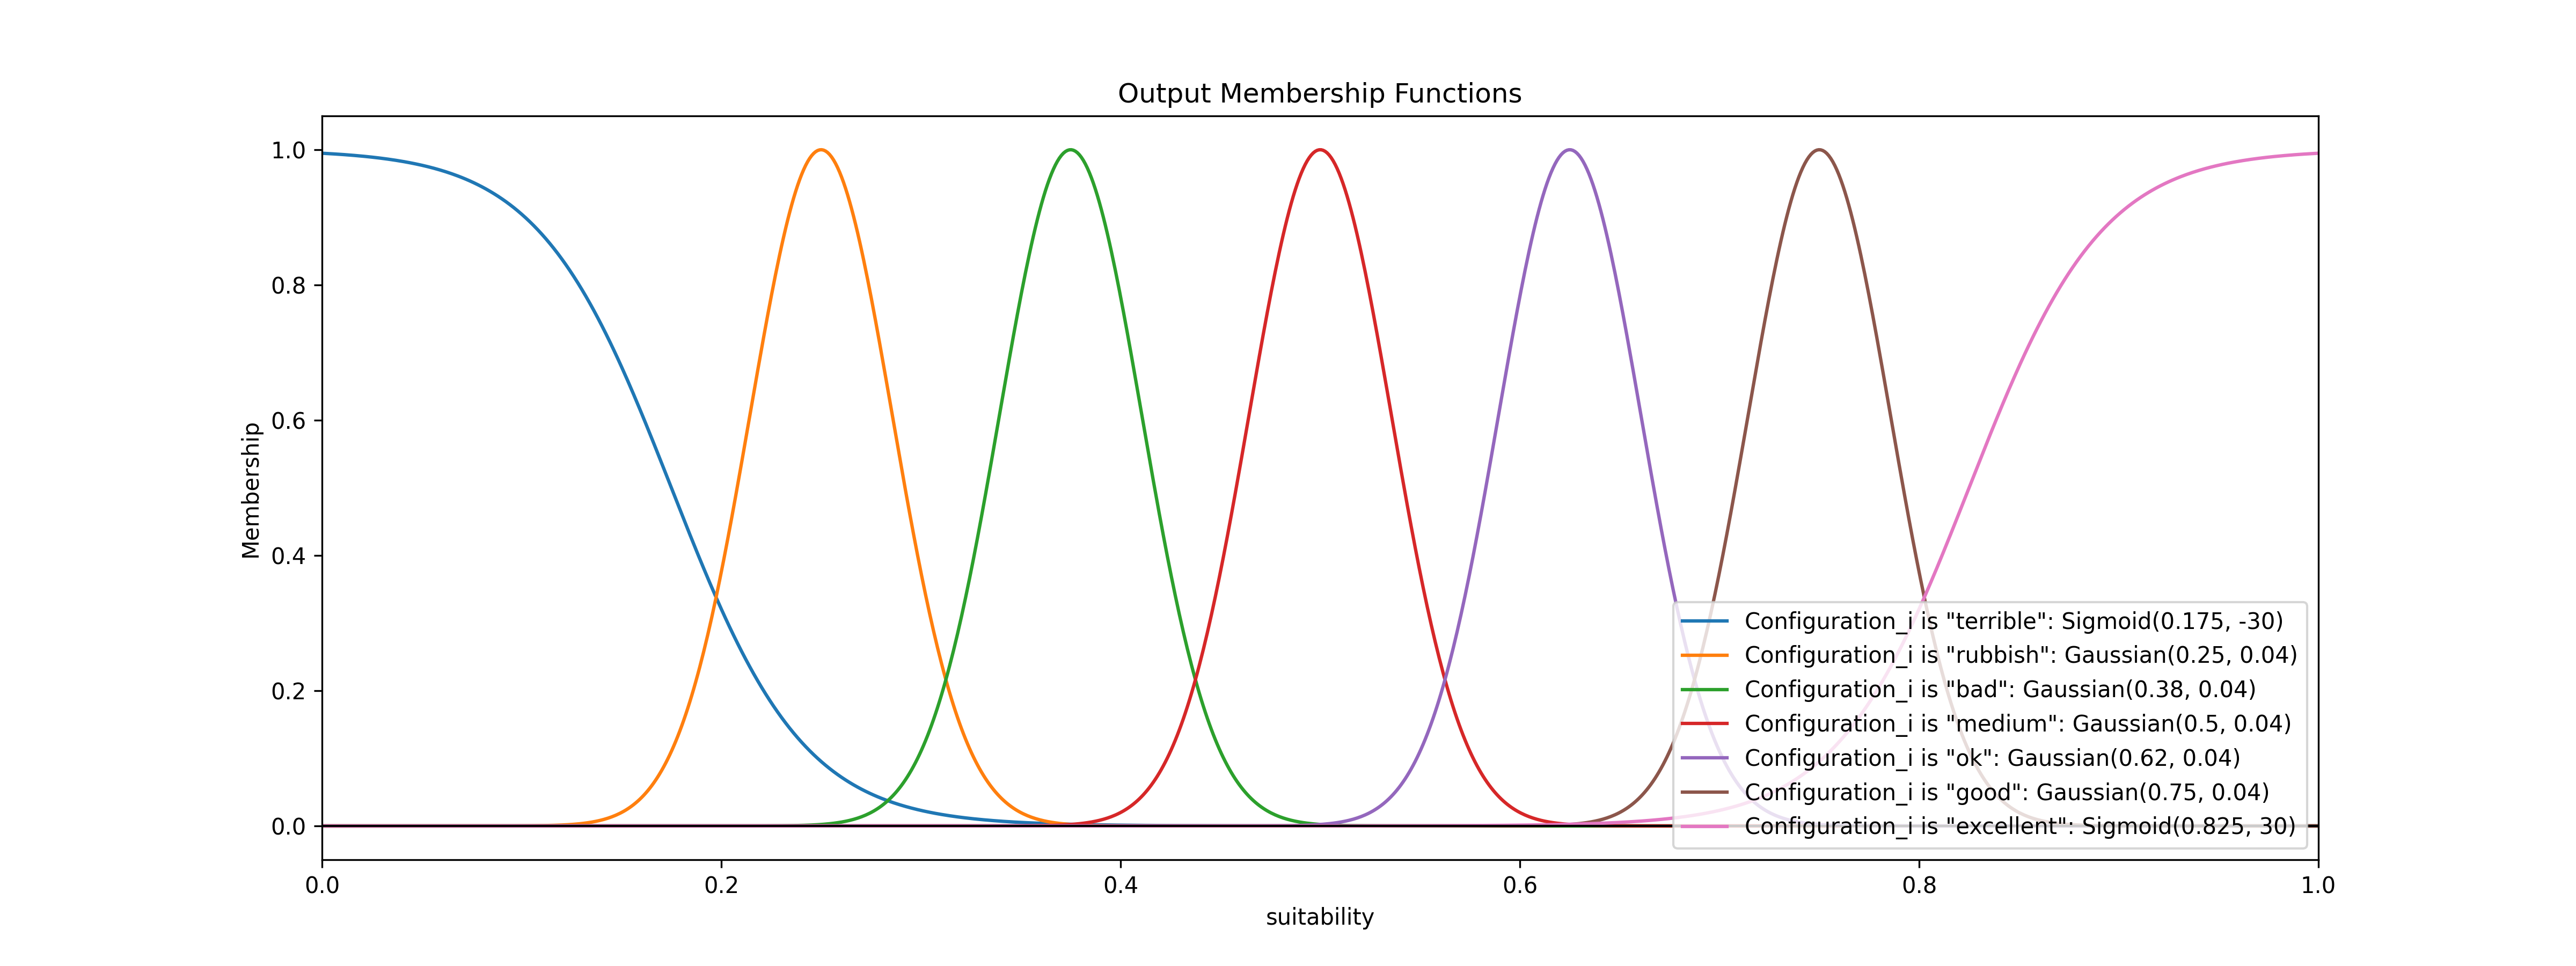
\includegraphics[width=\columnwidth,trim={1cm 0 2cm 1.5cm},clip]{figures/DataAnalytics/membership_suitability_config.png}
    \caption[Linguistic variable for the Suitability attribute]{
        Linguistic terms for the suitability variables. The fuzzy sets consist of  \texttt{sigmoid} membership functions at the borders and \texttt{gaussian} membership functions in the middle. The values are placed in coherent way. This time we will use the \gls{cog} defuzzification method and will make use of the interpolation between the values.
    }
    \label{fig:suitabilityLinguisticVariable}
\end{figure}


\begin{table}[H]
    \footnotesize
    \centering
    \begin{tabular}{|c|c|c|c|c|}
        \hline

        \textbf{LiveInfo Data} \footnote{
            The format of the LiveInfo tuple is: (avgParticlesPC, homogeneity, maxDensity,particlesPerCellStdDev, threadCount)
        }      & \textbf{Configuration} \footnote{
            The format of the Configuration is: Container, DataLayout, Traversal, Newton3
        }      & \textbf{Speedup}                  & \textbf{Suitability}          \\
        \hline
        \makecell{(0.905797,	0.035496,                                              \\	0.531948,	0.012989,	1) }                                                                                                              & \makecell{LinkedCells, AoS, lc\_sliced, enabled} &0.450641 & "bad"          \\
        \hline
        \makecell{(0.944637,	0.083797,                                              \\	0.691920	,	0.012989,	28) }                                                                                                              & \makecell{VerletClusterLists, AoS,vcl\_c06, disabled} &0.319094	 & "rubbish"          \\
        \hline
        \makecell{(0.944637,	0.079441,                                              \\	0.040082	,	0.012989,	12) }                                                                                                              & \makecell{LinkedCells, SoA,lc\_sliced, c02,enabled} &0.989101 & "excellent"          \\
        \hline

        \vdots & \vdots                            & \vdots               & \vdots \\
        \hline
    \end{tabular}
    \caption[Prepared training data for the Individual Tuning Approach]{Selection of the prepared training data for the Individual Tuning Approach. The table shows the liveinfo data and the corresponding prediction of top performing values for each tunable parameter. Each row represents a different tuning phase.}
    \label{tab:trainingDataSuitability}
\end{table}




\definecolor{LightCyan}{rgb}{0.88,1,1}
\newcolumntype{g}{>{\columncolor{LightCyan}}c}

\begin{table}[H]
    \footnotesize
    \centering
    \addtolength{\leftskip} {-3cm} % increase (absolute) value if needed
    \addtolength{\rightskip}{-3cm}

    \begin{tabular}{|c|c|c|c|g|}
        \multicolumn{4}{c}{\large{\textbf{Antecedent}}} & \multicolumn{1}{c}{\large{\textbf{Consequent}    }}                                                                                                                                             \\
        \hline
        \textbf{avgParticlesPC}                         & \textbf{homogeneity}                                & \textbf{particlesPCStdDev} & \textbf{threadCount}                              & \textbf{ LinkedCells\_AoS\_lc\_c01\_disabled} \\

        \hline
                                                        & \texttt{lower than 0.084}                           & \texttt{higher than 0.029} & \texttt{higher than 26.0 }                        & "medium"                                                 \\
        \hline
                                                        & \texttt{higher than 0.084}                          & \texttt{higher than 0.029} & \texttt{higher than 26.0 }                        & "bad"                                                    \\
        \hline
                                                        &                                                     & \texttt{higher than 0.02}  & \texttt{lower than 2.5	 }                          & "rubbish"                                                \\

        \hline
        \vdots                                          & \vdots                                              & \vdots                     & \vdots                                            & \vdots                                                   \\
        \hline

        \multicolumn{5}{c}{ }                                                                                                                                                                                                                             \\


        \multicolumn{4}{c}{\large{\textbf{Antecedent}}} & \multicolumn{1}{c}{\large{\textbf{Consequent}    }}                                                                                                                                             \\

        \hline
        \textbf{maxParticlesPerCell}                    & \textbf{homogeneity}                                & \textbf{particlesPCStdDev} & \textbf{threadCount}                              & \textbf{ LinkedCells\_AoS\_lc\_c04\_disabled} \\

        \hline
        \texttt{higher than 18.5	}                       & \texttt{lower than 0.082}                          &                            & \tabularCenterstack{c} {\texttt{higher than 18.0}                                                            \\ $\land$ \texttt{ lower than 26.0}} & "medium" \\

        \hline
        \texttt{higher than 18.5	}                       & \texttt{higher than 0.082}                          &                            & \tabularCenterstack{c} {\texttt{higher than 18.0}                                                            \\ $\land$ \texttt{ lower than 26.0}} & "bad" \\
        \hline


        \vdots                                          & \vdots                                              & \vdots                     & \vdots                                            & \vdots                                                   \\

        \hline
    \end{tabular}

    \caption[Extracted fuzzy rules for the Suitability Approach]{Extracted fuzzy rules for the Suitability Approach. The table shows a selection of the rules extracted from the decision trees trained on the training data in \autoref{tab:trainingDataSuitability}. The columns of the antecedent represent the different fuzzy sets taking part in the rule.}
    \label{tab:fuzzyRulesSuitability}
\end{table}




\begin{figure}[H]
    \centering
    \begin{tikzpicture}[scale=2,font=\small]
        \node[anchor=east] (L) at (-2,1.2) {$\text{LiveInfo} \in \mathbb{R}^d$};

        \foreach \x in {16,...,1}
            {
                \node [rectangle,rounded corners,draw,inner sep=2pt,fill=white!80!black, fill opacity=10/\x] (A) at (0+\x /16,0+\x/5) {
                    \begin{tikzpicture}[scale=2- \x/16 ,font=\tiny]
                        \begin{axis}%
                            [
                            title={FIS [Configuration\textsubscript {{\ifthenelse{\x<10}{\x\space}{\x}}]}},
                                    width=3.2cm,
                                    height=2cm,
                                    axis lines=center,
                                    xmin=0,
                                    xmax=4,
                                    xlabel={$\mathbb{R}$},
                                    x label style={at={(axis description cs:1,0.2)},anchor=west},
                                    ylabel=$\mu$,
                                    y label style={at={(axis description cs:0,0.8)},anchor=east},
                                    xtick={},
                                    xticklabels= {},
                                    ytick={},
                                    yticklabels={},
                                    ymax=1,
                                    every axis plot/.append style={thick},
                                    domain=0:4
                                ]
                            \addplot[blue, samples=17] {gaussian(x,1,0.2)};
                            \addplot[red,samples=15] {gaussian(x,2,0.2)};
                            \addplot[green,samples=17] {gaussian(x,3,0.2)};
                        \end{axis}
                    \end{tikzpicture}
                };

                \node (T) at (2.5+\x/35,0+\x/5) {
                    \begin{pgflowlevelscope}{\pgftransformscale{1-\x/28}}
                        suitability\textsubscript \x $\in \mathbb{R}$
                    \end{pgflowlevelscope}
                };

                \draw[->,ultra thick] (L.east) -- (A.west) ;
                \draw[->,ultra thick] (A) -- (T.west) ;
            }

    \end{tikzpicture}

    \caption[Visualization of the fuzzy inference systems for the Suitability Approach]{Selection of the fuzzy inference systems created from the fuzzy decision trees in \autoref{tab:fuzzyRulesSuitability}. Each fuzzy system is tailored to evaluate a specific configuration and maps the LiveInfo data to a suitability value representing the predicted performance of the configuration. There are as many fuzzy systems as there are possible configurations.}

    \label{fig:fuzzyInferenceSystemSuitability}
\end{figure}


